% ============================================================================
%  BRAVE-Based Real-Time Voice-to-Instrument Resynthesis
%  Final memoir, TFG, Grau en Enginyeria de Sistemes Audiovisuals
%  Universitat Pompeu Fabra, Escola Superior Politecnica
%  Author: Jofre Geli de Fuenmayor             Submission: 12 June 2026
%
%  NOTE: This file mirrors the structure of the UPF DTIC TFG template
%  (tfg_dtic_upf.cls, derived from book). To compile under the official
%  class, replace the documentclass line below with
%      \documentclass{tfg_dtic_upf}
%  and ensure tfg_dtic_upf.cls and logo_upf.png are in the same folder.
% ============================================================================

\documentclass[a4paper,11pt,oneside,openany]{book}

% --- Encoding and language ---------------------------------------------------
\usepackage[T1]{fontenc}
\usepackage[utf8]{inputenc}
\usepackage[main=english,catalan,spanish]{babel}

% --- Page geometry (matches tfg_dtic_upf log: ~2.5cm margins, twoside) -------
\usepackage[a4paper,top=2.5cm,bottom=2.5cm,left=2.5cm,right=2.5cm]{geometry}

% --- Fonts and microtypography -----------------------------------------------
\usepackage{times}
\usepackage{microtype}

% --- Math, units, tables, figures --------------------------------------------
\usepackage{amsmath,amssymb}
\usepackage{siunitx}
\usepackage{booktabs}
\usepackage{tabularx}
\usepackage{multirow}
\usepackage{graphicx}
\usepackage{float}
\usepackage{caption}
\usepackage{subcaption}
\usepackage{xcolor}
\usepackage{tikz}
\usetikzlibrary{positioning,arrows.meta,fit,calc,shapes.geometric}

% --- Code listings -----------------------------------------------------------
\usepackage{listings}
\lstset{
  basicstyle=\ttfamily\footnotesize,
  breaklines=true,
  frame=single,
  captionpos=b,
  showstringspaces=false
}

% --- Bibliography (APA, biblatex+biber) --------------------------------------
\usepackage{csquotes}
\usepackage[backend=biber,style=apa,sortcites=true,sorting=nyt]{biblatex}
\addbibresource{references.bib}

% --- Indexing and appendices --------------------------------------------------
\usepackage{makeidx}
\usepackage[titletoc]{appendix}
\makeindex

% --- Hyperlinks --------------------------------------------------------------
\usepackage{hyperref}
\hypersetup{
  colorlinks=true,
  linkcolor=black,
  citecolor=blue,
  urlcolor=blue,
  pdftitle={BRAVE-Based Real-Time Voice-to-Instrument Resynthesis},
  pdfauthor={Jofre Geli de Fuenmayor}
}

% --- Metadata ----------------------------------------------------------------
\newcommand{\thesisTitle}{BRAVE-Based Real-Time Voice-to-Instrument Resynthesis}
\newcommand{\thesisSubtitle}{System Design, Training Diagnostics, and Failure Analysis}
\newcommand{\thesisAuthor}{Jofre Geli de Fuenmayor}
\newcommand{\thesisAdvisor}{Lonce Wyse \& Xavier Lizarraga}
\newcommand{\thesisInstitution}{Universitat Pompeu Fabra}
\newcommand{\thesisFaculty}{Escola Superior Polit\`ecnica}
\newcommand{\thesisDegree}{Grau en Enginyeria de Sistemes Audiovisuals}
\newcommand{\thesisDate}{Juny 2026}

% --- Captions, paragraph spacing --------------------------------------------
\captionsetup{font=small,labelfont=bf,format=plain}
\setlength{\parindent}{0pt}
\setlength{\parskip}{6pt}

% ============================================================================
\begin{document}
\frontmatter

% --- Title page --------------------------------------------------------------
\begin{titlepage}
\centering
\vspace*{1cm}
% Logo placeholder (uncomment when logo_upf.png is available)
% 
\includegraphics[width=0.45\textwidth]{logo_upf.png}\\[2cm]
{\Large \textsc{\thesisInstitution}\\\thesisFaculty}\\[3cm]
{\Huge\bfseries \thesisTitle\par}\vspace{0.6cm}
{\Large\itshape \thesisSubtitle\par}\vspace{3cm}
{\Large\textbf{\thesisAuthor}}\\[0.2cm]
Treball Fi de Grau\\
\thesisDegree\\[2cm]
Director: \thesisAdvisor\\[3cm]
\thesisDate
\end{titlepage}

% --- Abstracts ---------------------------------------------------------------
\chapter*{Abstract}
\addcontentsline{toc}{chapter}{Abstract}
This thesis investigates whether the streaming-causal BRAVE architecture can deliver voice-driven instrument resynthesis at sub-10 ms latency when trained on heterogeneous, limited-scale public datasets. Six guitar iterations (v1--v6) and two drum iterations (drums\_v1, drums\_v2) were systematically trained and evaluated under a custom diagnostic framework. The principal outcome is a guitar autoencoder (guitar\_v6, mid-Phase-2 epoch 1935) that reconstructs in-distribution guitar audio but does not generalise to voice: vocal input lies outside the guitar training distribution (out-of-distribution) and was not rendered as recognisable guitar by any iteration. A separate attempt to reuse the successful guitar\_v6 configuration template for a drums model did not transfer cleanly, with adversarial training destabilising before completion. Comparison against an external baseline (the official ACIDS-IRCAM percussion model) showed it to be more responsive than our drums\_v1 model by more than two orders of magnitude on the same synthetic-input diagnostic (forward difference 1.75 versus 0.0045), indicating that the out-of-distribution limitation is a consequence of training-recipe and data-scale choices rather than a fundamental architectural constraint of BRAVE. The principal contributions are a five-mode failure taxonomy for RAVE-family models trained on small corpora, a cross-checkpoint calibration of the spectral-correlation diagnostic that exposes a previously unreported limitation of that metric, and an external-baseline validation that disentangles architectural from training-recipe sources of failure. The thesis pivots mid-project from a single-prototype demonstration goal to a documented case-study and failure-analysis investigation, an honest realignment given the data-scale limits encountered.

\chapter*{Resum}
\addcontentsline{toc}{chapter}{Resum}
\selectlanguage{catalan}%
Aquesta tesi investiga si l'arquitectura BRAVE de tipus causal-streaming pot oferir resíntesi d'instruments controlada per veu amb una latència inferior a 10 ms quan s'entrena sobre conjunts de dades públics, heterogenis i de mida limitada. S'han entrenat sis iteracions de guitarra (v1--v6) i dues de bateria (drums\_v1, drums\_v2), avaluades amb un marc diagnòstic propi. El principal resultat és un autoencoder de guitarra (guitar\_v6, època 1935 a la meitat de la Fase 2) que reconstrueix àudio de guitarra en distribució però no generalitza a la veu: l'entrada vocal queda fora de la distribució d'entrenament de guitarra (out-of-distribution) i cap iteració no la va reproduir com a guitarra recognoscible. Un intent a part de reutilitzar la plantilla de configuració de guitar\_v6 per a un model de bateria no es va transferir netament, amb l'entrenament adversari desestabilitzant-se abans de completar-se. La comparació amb una línia base externa (el model de percussió preentrenat oficial ACIDS-IRCAM) la va mostrar més responsiva que el nostre model drums\_v1 per més de dos ordres de magnitud en el mateix diagnòstic d'entrada sintètica (diferència de propagació 1.75 enfront de 0.0045), indicant que la limitació OOD és conseqüència de la recepta d'entrenament i de l'escala de dades més que d'una restricció arquitectònica fonamental de BRAVE. Les contribucions principals són una taxonomia de cinc modes de fallada per als models de la família RAVE entrenats amb corpus petits, una calibració entre punts de control de la mètrica de correlació espectral que exposa una limitació no documentada prèviament d'aquesta mètrica, i una validació mitjançant línia base externa que diferencia les causes arquitectòniques de les de recepta d'entrenament.
\selectlanguage{english}%

\chapter*{Resumen}
\addcontentsline{toc}{chapter}{Resumen}
\selectlanguage{spanish}%
Esta tesis investiga si la arquitectura BRAVE de tipo causal-streaming puede ofrecer resíntesis de instrumentos controlada por voz con una latencia inferior a 10 ms cuando se entrena sobre conjuntos de datos públicos, heterogéneos y de tamaño limitado. Se entrenaron sistemáticamente seis iteraciones de guitarra (v1--v6) y dos de batería (drums\_v1, drums\_v2), evaluadas bajo un marco diagnóstico propio. El resultado principal es un autoencoder de guitarra (guitar\_v6, época 1935 a mitad de la Fase 2) que reconstruye audio de guitarra en distribución pero no generaliza a la voz: la entrada vocal queda fuera de la distribución de entrenamiento de guitarra (out-of-distribution) y ninguna iteración la reprodujo como guitarra reconocible. Un intento aparte de reutilizar la plantilla de configuración de guitar\_v6 para un modelo de batería no se transfirió limpiamente, con el entrenamiento adversario desestabilizándose antes de completarse. La comparación con una línea base externa (el modelo de percusión preentrenado oficial ACIDS-IRCAM) lo mostró más responsivo que el modelo drums\_v1 por más de dos órdenes de magnitud en el mismo diagnóstico de entrada sintética (diferencia de propagación 1.75 frente a 0.0045), indicando que la limitación OOD es consecuencia de la receta de entrenamiento y la escala de datos más que de una restricción arquitectónica fundamental de BRAVE. Las contribuciones principales son una taxonomía de cinco modos de fallo para modelos de la familia RAVE entrenados con corpus pequeños, una calibración entre puntos de control de la métrica de correlación espectral que expone una limitación no documentada previamente de dicha métrica, y una validación mediante línea base externa que distingue las causas arquitectónicas de las relativas a la receta de entrenamiento.
\selectlanguage{english}%

% --- Acknowledgements (stub) -------------------------------------------------
\chapter*{Acknowledgements}
\addcontentsline{toc}{chapter}{Acknowledgements}
The author would like to thank the project director, \thesisAdvisor, for guidance throughout the iterative development and for the methodological flagging of the dataset heterogeneity concern that shaped Decision~3 (Appendix~D). Acknowledgement is also due to the ACIDS-IRCAM research group for releasing the RAVE and BRAVE architectures, training code, and pretrained checkpoints used as the project's external baseline, and to the maintainers of the GuitarSet, Guitar-TECHS, IDMT-SMT-Guitar and Groove MIDI Dataset corpora.

% --- Tables of contents, figures, tables -------------------------------------
\tableofcontents
\listoffigures
\listoftables

\mainmatter

% ============================================================================
%  CHAPTER 1 -- INTRODUCTION
% ============================================================================
\chapter{Introduction}\label{chap:intro}

\section{Motivation}\label{sec:motivation}

Currently, in the world of live electronic music performance, there is a tendency to use deep neural models to control timbre in a very expressive way. The human voice is a very expressive, natural and simple way to control such systems and does not need any special equipment except a microphone.

Neural audio synthesis is now advancing thanks to key models such as WaveNet \parencite{vandenoord2016wavenet}, NSynth \parencite{engel2017nsynth}, and DDSP \parencite{engel2020ddsp}. However, these initial models are not very suitable for live use. Autoregressive models require a lot of computing power, and on the other hand, early differentiable signal processing models often have to focus on explicit tone tracking or processing in windows that can cause noticeable lag.

The launch of RAVE \parencite{caillon2021rave} became highly influential, facilitating high-quality synthesis even on widely accessible CPU hardware. BRAVE \parencite{caspe2025brave} goes a step further with a streaming-causal architecture aimed at creating interactive and responsive music in real-time. However, converting voice to instrument is quite difficult when the source and destination timbres are very different acoustically. For example, plucked string instruments, such as the guitar, have a sharp percussive attack and an exponentially decaying envelope, which is very different from the sustained, formant-rich structure of the human voice. This work investigates whether streaming-causal systems can achieve voice-to-guitar resynthesis that is subjectively plausible as guitar, at a target latency of 10\,ms or less so it is usable in live performance. Addressing this cross-modal mismatch is crucial to the enhancement of music interfaces that enable human vocal intuition to be the foundation for machine synthesis.

\section{Research Questions}\label{sec:research_questions}

The motivation above frames a problem domain rather than a tightly defined investigation. To make the scope of the work explicit and to give the methodology of Chapter~\ref{chap:methodology} and the evaluation of Chapter~\ref{chap:results} something concrete to answer, the project is organised around three research questions:

\begin{description}
\item[RQ1 \textnormal{(Feasibility).}] Can a streaming-causal variational autoencoder of the RAVE/BRAVE family be trained on small, open instrument corpora (under twenty hours per instrument) to operate as a real-time autoencoder at sub-10\,ms end-to-end latency on a single consumer GPU, using a reproducible Windows-based toolchain?
\item[RQ2 \textnormal{(Cross-modal generalisation).}] Does an instrument-domain-only autoencoder's learned latent manifold generalise to out-of-distribution vocal excitation at inference time, in the absence of any paired voice-to-instrument training data?
\item[RQ3 \textnormal{(Failure diagnosis).}] What training instabilities and degenerate behaviours emerge under these constrained training conditions, and to what extent can each be diagnosed from in-training metrics and synthetic-input probes alone, without recourse to formal perceptual evaluation?
\end{description}

RQ1 and RQ3 are answered constructively across the iteration sequence reported in Chapter~\ref{chap:results}: a working in-distribution guitar autoencoder is obtained and five distinct training-failure modes are isolated. RQ2 is answered negatively, in a qualified form: instrument-only training did not yield perceptually convincing voice-to-instrument resynthesis on the small open corpora used here, and the IRCAM percussion baseline (\S\ref{sec:ircam_baseline}) suggests this is a training-recipe and data-scale limitation rather than an architectural impossibility.

\section{Objectives and Scope}\label{sec:objectives}

To address the research question, this project defines a general objective to design and evaluate a streaming neural resynthesis pipeline for expressive voice-driven instrumental synthesis. The investigation is organised according to the following specific objectives:

\begin{itemize}
\item Examine whether it is possible to keep the total latency below 10\,ms in a visual programming environment with a causal Variational Autoencoder (VAE) architecture.
\item Assess the performance of instrument-specific models when driven by both vocal percussive inputs and sustained tonal singing.
\item Document training instabilities and failure modes throughout the RAVE/BRAVE architecture family.
\item Evaluate the limits of audio reconstruction fidelity when models are presented with out-of-distribution vocal signals.
\end{itemize}

The scope of this project is restricted to monophonic audio resynthesis since this constraint lowers computational complexity and also enables stable inference on consumer-grade devices. Consequently, polyphonic modelling, offline batch processing, and linguistic speech conversion (text-to-speech) are considered out-of-scope.

\section{Methodology}\label{sec:intro_methodology}

The approach combined iterative system implementation with structured diagnostic protocols. The methodology, detailed in Chapter~\ref{chap:methodology}, is organised around four operational axes --- system architecture, training paradigm, dataset preparation, and diagnostic protocols --- operationalised through the following five processes:

\begin{enumerate}
\item \textbf{Dataset preparation:} Public guitar and drum-kit corpora were preprocessed to a uniform 44.1\,kHz mono format. This stage included a quantitative analysis of noise-floor heterogeneity to identify potential biases in the training data.
\item \textbf{Training procedure:} Models were trained under a two-step procedure: an independent representation learning phase optimising a multi-scale STFT loss, followed by adversarial fine-tuning intended to improve perceptual naturalness.
\item \textbf{Deployment:} The trained TorchScript models were integrated into Pure Data through the \texttt{nn\textasciitilde} external, supporting live vocal interaction at a 64-sample block size.
\item \textbf{Quantitative evaluation:} The main focus was using end-to-end latency benchmarks together with synthetic-input diagnostic probes (\S\ref{sec:diagnostic_method}). The degree of alignment between input and output Short-Time Fourier Transform (STFT) magnitudes was also considered as a metric for spectral reconstruction closeness.
\item \textbf{Qualitative testing:} Listening evaluation at each checkpoint was conducted informally by the author. No formal MUSHRA or MOS test with multiple participants was administered; the implications of this evaluation design are stated explicitly in \S\ref{sec:diagnostic_method} and \S\ref{sec:method_limitations} rather than deferred to the conclusions.
\end{enumerate}

\section{Original Contributions}\label{sec:contributions}

The following are the original contributions of this work. Each is grounded in the experimental evidence reported in Chapter~\ref{chap:results} and the methodological framework of Chapter~\ref{chap:methodology}:

\begin{itemize}
\item \textbf{Original contribution 1 --- Failure-mode taxonomy.} A systematic, evidence-anchored account of five distinct training-failure modes observed across an eight-iteration training sequence: posterior collapse (v1), latent underutilisation (v2), discriminator dominance / generator mode collapse (v3, v4, drums\_v2), discriminator collapse (v5), and out-of-distribution decoder behaviour (v6, drums\_v1). The author is not aware of a published RAVE/BRAVE study that traces this many distinct failure modes within a single training programme.
\item \textbf{Original contribution 2 --- Calibration of the STFT-magnitude-correlation diagnostic.} A cross-checkpoint calibration study (\S\ref{sec:stft_calibration}, Table~\ref{tab:stft_calibration}) showing that the STFT-magnitude-correlation metric initially proposed as a working acceptance heuristic does not robustly discriminate working autoencoders from collapsed ones, because collapsed checkpoints produce trivially correlated near-silent outputs. This is a methodological finding that constrains how the metric should be used in future replication work.
\item \textbf{Original contribution 3 --- External-baseline disentanglement.} A side-by-side diagnostic comparison between drums\_v1 and the official ACIDS-IRCAM percussion checkpoint (\S\ref{sec:ircam_baseline}) measured under identical conditions in Pure Data, isolating the observed OOD limitation as a training-recipe and dataset-scale issue rather than an architectural impossibility.
\item \textbf{Original contribution 4 --- Working in-distribution guitar autoencoder.} A streaming-causal RAVE v2 guitar autoencoder (\texttt{guitar\_v6\_best.ts}) recovered from a sequence of failed iterations, used as the reference point against which cross-modal vocal input is evaluated.
\item \textbf{Original contribution 5 --- Dataset-heterogeneity quantification.} A noise-floor analysis (\S\ref{sec:noise_floor}, Table~\ref{tab:noise_floor}) measuring a 35.9\,dB spread across six recording paths within the consolidated guitar corpus, with documented implications for what features the encoder is likely to internalise as salient.
\item \textbf{Original contribution 6 --- Open, reproducible Windows pipeline.} A version-controlled training, evaluation, and deployment pipeline (preprocessing, four \texttt{acids-rave} compatibility patches, training launchers, diagnostic and figure-generation scripts, Pure Data patches) released alongside this thesis so that the eight reported iterations can be re-run on commodity Windows hardware.
\end{itemize}

\section{Document Structure}\label{sec:doc_structure}

The thesis is organised into six chapters. Chapter~\ref{chap:sota} reviews the state of the art in neural synthesis and timbre transfer. Chapter~\ref{chap:methodology} details the methodology, focusing on system architecture and training protocols. Chapter~\ref{chap:implementation} describes the implementation of the Pure Data environment and the software pipeline. Chapter~\ref{chap:results} presents the evaluation results, including the failure taxonomy, the external-baseline validation, and the dataset heterogeneity analysis. Chapter~\ref{chap:conclusions} summarises the findings and proposes future work across calibrated latency measurement, formal perceptual evaluation, RAVE v3 architectures, mixed-domain training data, hybrid pipelines, and replication on larger corpora. Technical configurations, the project planning artefacts (Project Charter and Gantt), and code references are provided in the appendices.

% ============================================================================
%  CHAPTER 2 -- STATE OF THE ART
% ============================================================================
\chapter{State of the Art}\label{chap:sota}

Over the past decade, the field of neural audio synthesis has shifted from slow autoregressive models toward streaming-causal architectures capable of producing music in real time. This chapter is structured around three topics: (i)~the architectural genealogy from WaveNet to BRAVE, (ii)~methods of timbre transfer and voice conversion, and (iii)~datasets used to train and test these models. The chapter finishes by clearly indicating the gaps in research that the present work aims to fill.

\paragraph{Literature selection methodology.} The works discussed have been chosen based on three factors: (a)~direct architectural relevance to the streaming-causal Variational Autoencoders (VAEs) used in this work, (b)~methodological relevance to cross-modal timbre transfer, and (c)~additional contributions to GAN stability and audio reconstruction quality that influenced the RAVE v2 architecture. Priority was given to highly ranked conference and journal venues (NeurIPS, ICML, ICLR, ISMIR, ICASSP) and arXiv preprints were used when they are the canonical reference for a widely used architecture. The literature search was conducted from March to May 2026. As a limitation of this survey, streaming neural audio synthesis is a fast-evolving field; some very recent architectures are mainly documented through preprints and open-source implementations rather than peer-reviewed publications, and the canonical citation of several systems used in this project (most notably BRAVE) is an arXiv preprint.

\section{Neural Audio Synthesis Architectures}\label{sec:nas_arch}

\subsection*{Early Neural Synthesis Architectures}

WaveNet \parencite{vandenoord2016wavenet}, an autoregressive model factorising the joint probability of the waveform into a product of conditional probabilities and generating audio sample by sample, laid the groundwork for modern neural audio synthesis. WaveNet achieved levels of naturalness in text-to-speech tasks that were unprecedented at the time, but live usage is impractical because every single audio sample requires a full forward pass through the network. NSynth \parencite{engel2017nsynth} applied the same architectural family to musical notes by training a WaveNet autoencoder on more than 300,000 one-note sound samples. The authors demonstrated a 16-dimensional temporal embedding representation that captures the semantic timbral qualities of sounds and allows morphing from one instrument identity to another. NSynth still inherits the autoregressive bottleneck of WaveNet and is restricted to isolated notes rather than continuous performance.

\subsection*{Differentiable Signal Processing}

Differentiable Digital Signal Processing (DDSP) \parencite{engel2020ddsp} introduced a different perspective. Rather than outputting raw audio samples, DDSP places conventional DSP modules (harmonic additive synthesisers and filtered noise) directly into the computation graph and trains a neural network to produce their control parameters. The inductive bias of these synthesisers leads to significant reductions in data and model-size requirements compared with autoregressive models. The trade-off is that DDSP depends on explicit fundamental-frequency (F0) and loudness signals to perform inference; in a live performance setting, this entails an ongoing dependence on an external pitch-estimation module on the critical path.

\subsection*{Variational Autoencoders for Raw Audio: The RAVE Architecture}

Whereas WaveNet and DDSP improve reconstruction by operating directly on the raw waveform, the Variational Autoencoder model \parencite{kingma2013vae} suggests learning structured latent variables usable both for accurate reconstruction and for new data generation. RAVE \parencite{caillon2021rave} brings this theory into practice for real-time audio.

\textbf{Two-stage training pipeline.} RAVE first trains a VAE and then adversarially fine-tunes it. In Phase~1, a multi-scale STFT loss trains the encoder--decoder pair to minimise spectral reconstruction error \parencite{engel2020ddsp,caillon2021rave}. In Phase~2, the encoder is frozen and the decoder is trained to fool a multi-scale waveform discriminator \parencite{goodfellow2014gan,kong2020hifigan}, enhancing the perceptual quality of the output.

\textbf{Multi-band decomposition for real-time inference.} To enable real-time inference on typical CPU hardware, RAVE uses a 16-band frequency decomposition based on a Pseudo-Quadrature Mirror Filter (PQMF) bank \parencite{cruzroldan2002pqmf}. This decomposes the signal into sixteen subbands, effectively reducing the per-band processing rate prior to the encoding step \parencite{caillon2021rave}.

\textbf{Adversarial stabilisation techniques.} Stability of the adversarial phase depends on additional techniques from the generative-modelling literature: spectral normalisation of the discriminator \parencite{miyato2018spectralnorm}, multi-period discriminators inherited from HiFi-GAN \parencite{kong2020hifigan}, and multi-scale spectral losses computed over different STFT window sizes \parencite{engel2020ddsp}. Together, these strategies have established RAVE as one of the most widely adopted neural timbre-transfer architectures for interactive applications.

\subsection*{Streaming-Causal Extension: BRAVE}

Standard RAVE operates with non-causal convolutional layers, and its end-to-end latency was measured at tens of milliseconds \parencite{caillon2021rave}, a delay likely to disrupt live musical performance. BRAVE \parencite{caspe2025brave} redesigns RAVE for streaming inference. The most important architectural modifications are: replacing non-causal convolutions with causal ones, reducing the encoder's compression factor to limit accumulated group delay, and relaxing the PQMF attenuation specification to shorten the filter taps. Causal convolutions are the central enabler: by removing the requirement of future temporal context, they allow inference to run stepwise on streaming audio without buffering ahead of the current sample. Combined with cached convolutional state and a specialised C++ inference path, these modifications achieve a reported audio-to-audio latency below 10\,ms while preserving the qualitative characteristics of RAVE \parencite{caspe2025brave}.

SoundStream \parencite{zeghidour2022soundstream}, a neural codec developed in parallel, independently showed that convolutional encoder--decoder topologies could be used for low-latency streaming when padding schemes are designed carefully, providing architectural justification for BRAVE's causal design. A trade-off acknowledged by the BRAVE authors is that the limited temporal context can degrade pitch accuracy at extreme registers for melodic instruments.

\subsection*{Diffusion-Based Audio Synthesis}\label{subsec:diffusion}

The past two years have seen the emergence of latent diffusion architectures adapted to general audio and music generation, including AudioLDM \parencite{liu2023audioldm}, MusicGen \parencite{copet2023musicgen}, MAGNeT \parencite{ziv2024magnet} and Stable Audio \parencite{evans2024stableaudio}. These models achieve state-of-the-art reconstruction quality and have substantially expanded the range of text-conditioned and inpainting tasks that can be demonstrated on contemporary hardware. They are excluded from the present comparison for two reasons. First, their inference cost is typically too computationally expensive for sub-10\,ms interactive deployment, even with accelerated samplers, which precludes streaming use. Second, their conditioning interfaces --- natural-language prompts, instrument-class labels or melody contours --- are orthogonal to the continuous, voice-driven control that motivates the present project. Diffusion-based approaches remain an open research direction for offline cross-modal resynthesis and are revisited as future work in \S\ref{sec:future_work}.

\subsection*{Synthesis: An Architectural Evolution Shaped by Latency}\label{subsec:arch_synthesis}

Considered consecutively, these architectures form a distinct evolutionary path. WaveNet was the first to show that a neural network could generate waveforms directly and realistically, but it could only operate offline. DDSP enabled real-time inference by giving up the freedom of generating raw waveforms in favour of an inductive bias toward DSP-based synthesis, but at the cost of requiring an external pitch-estimation stage. RAVE removed the need for explicit pitch conditioning by discovering the latent space directly, but its non-causal context kept latency above the level of perceptual immediacy for live use. BRAVE brings inference down to the sub-10\,ms regime by accepting an even smaller temporal context, the latest step in a decade-long progression away from offline waveform modelling and toward interactive musical instruments. Diffusion-based models represent a parallel branch oriented toward offline high-quality generation rather than real-time interaction.

\paragraph{Project architectural choice.} BRAVE is the only architecture among those reviewed that simultaneously meets the three major constraints of the project: implicit pitch modelling (eliminating the need for an external pitch tracker on the audio path), streaming inference, and sub-10\,ms end-to-end latency. WaveNet and NSynth are excluded by their autoregressive nature; DDSP by its reliance on external pitch tracking; standard RAVE by its non-causal context; and the diffusion family by inference cost. The methodology and assessment in Chapters~\ref{chap:methodology} and~\ref{chap:results} are therefore based on BRAVE. Table~\ref{tab:arch_comparison} summarises the comparison.

\begin{table}[H]
\centering
\caption{A concise comparison of the architectures analysed in \S\ref{sec:nas_arch}. Latency is the end-to-end audio-to-audio delay as measured and reported by respective authors on their cited hardware configurations; entries without a directly measurable latency are qualitatively discussed.}
\label{tab:arch_comparison}
\footnotesize
\setlength{\tabcolsep}{4pt}
\renewcommand{\arraystretch}{1.2}
\begin{tabularx}{\textwidth}{@{}>{\raggedright\arraybackslash}p{2.3cm}ccXXXX@{}}
\toprule
\textbf{Model} & \textbf{Real-time} & \textbf{Causal} & \textbf{Latency} & \textbf{Pitch conditioning} & \textbf{Latent representation} & \textbf{Main limitation for live voice use} \\
\midrule
WaveNet (2016) & No & Yes & Minutes per second of audio & Optional (linguistic) & None (direct waveform) & Sample-by-sample generation prohibits live use \\
NSynth (2017) & No & Yes & Minutes per second of audio & None & 16-D temporal embedding & Restricted to isolated notes \\
DDSP (2020) & Yes & No & Real-time; bounded by pitch tracker & Explicit F0 + loudness & Explicit DSP control parameters & External pitch tracker on critical path \\
TimbreTron (2018) & No & No & Offline (CQT + WaveNet vocoder) & Implicit via CQT & CQT spectrogram & Spectrogram-domain inference too slow \\
RAVE (2021) & Yes & No & $\sim$50\,ms reported & Implicit & Learned VAE latent & Non-causal context limits perceptual immediacy \\
\textbf{BRAVE (2025)} & \textbf{Yes} & \textbf{Yes} & $<10$\,ms reported & Implicit & Learned VAE latent (causal) & Shorter temporal context can degrade pitch at extremes \\
Diffusion family (2023--2024) & No & No & Seconds to minutes per second of audio & Text / class / melody & Latent diffusion & Inference cost prohibits streaming use \\
\bottomrule
\end{tabularx}
\end{table}

\paragraph{Pretrained ACIDS-IRCAM checkpoints.} Beyond the published architectural descriptions surveyed above, the ACIDS-IRCAM group distributes a library of pretrained RAVE-family checkpoints (percussion, darbouka, voice, violin, electric guitar, and others) accessible through the ACIDS RAVE-VST API \parencite{acidsircam2024models}. These checkpoints were trained on larger and, where reported, more curated corpora than the open datasets reviewed in \S\ref{sec:nas_datasets}, although their exact training configurations are not published alongside the released weights. In Chapter~\ref{chap:results} the official percussion checkpoint is used as an external baseline against which the responsiveness of the present project's drum-trained model is calibrated, in order to disentangle architectural from training-recipe contributions to the out-of-distribution voice limitation observed in this work.

\section{Timbre Transfer and Voice Conversion}\label{sec:timbre_transfer}

The trajectory in \S\ref{sec:nas_arch} is concerned with creating audio from a learned distribution. Converting one sound into the timbre of another has a related but distinct literature that predates RAVE and that nonetheless points to the cross-modal problems addressed by this thesis.

\subsection*{Definition of Timbre}

Classically, timbre is the perceptual characteristic that differentiates two sounds having the same pitch and loudness. It is usually treated as a multidimensional notion encompassing spectral envelope, attack and decay characteristics, fine-grained temporal modulations, and the resonant properties of the source. In machine learning, timbre transfer is the conversion of the timbral features of a source signal into those of a target instrument while preserving musical elements such as pitch, rhythm, and dynamics.

\subsection*{Spectrogram-Domain Transfer}

The first demonstrations of high-quality musical timbre transfer were given by TimbreTron \parencite{huang2018timbretron}, which uses CycleGAN, an image-to-image translation network, on constant-Q transform (CQT) spectrograms. CQT representations have approximate pitch equivariance, which makes them suitable for music. TimbreTron solves the phase-reconstruction problem associated with spectrogram-domain approaches by attaching a conditional WaveNet vocoder to convert the transferred CQT to a waveform. The method produces convincing piano-to-harpsichord and similar conversions but cannot be used live because of WaveNet's offline inference time.

\subsection*{Voice Conversion}

Voice conversion (VC) is concerned with changing the speaker identity while preserving the spoken content. AutoVC \parencite{qian2019autovc} proposed an autoencoder-only model in which an information bottleneck separates speaker-dependent features from phonetic content, making zero-shot transfer possible even for target speakers not seen during training. Neural audio codecs such as SoundStream \parencite{zeghidour2022soundstream} take the encoder--decoder framework further by performing general audio compression with residual vector quantisation, achieving very high reconstruction quality at low bitrates.

\subsection*{Vocal Percussion Transcription}\label{subsec:vpt}

A parallel line of work concerns the discrete classification of beatbox and other vocal percussion sounds into drum-instrument categories (kick, snare, hi-hat, cymbal). Early systems relied on spectral and timbral features combined with classical machine-learning classifiers \parencite{stowell2008beatboxing}. Subsequent work introduced labelled corpora --- most notably the Amateur Vocal Percussion (AVP) dataset \parencite{delgado2019avp}, which provides 9780 onset-aligned, four-class vocal-percussion utterances from 28 participants --- and shifted to convolutional networks operating on short audio windows. Vocal-percussion transcription is methodologically orthogonal to the timbre-transfer task that frames the present thesis: it produces symbolic onset-class labels rather than a continuous resynthesised waveform. The two approaches are, however, naturally combinable into hybrid pipelines that route classified onsets to per-class neural synthesisers or sample banks; this combination is identified as a future-work direction in \S\ref{sec:future_work}.

\subsection*{The Voice-to-Instrument Cross-Modal Gap}\label{subsec:cross_modal_gap}

The distance between voice-to-voice and voice-to-instrument tasks is substantial. Voice production is characterised by a formant structure generated by the vocal tract and phonetic content communicated through rapid articulation. A plucked-string instrument such as a guitar, on the other hand, derives its sound from mechanical excitation, body resonance and an exponentially decaying envelope; such instruments do not produce formants and have no phonetic content. If a VAE is trained solely on guitars, its latent-space manifold is therefore expected to be poorly aligned with vocal features \parencite{kingma2013vae,caillon2021rave}. Whether the encoder can position the voice within a meaningful region of that manifold, and whether the decoder can generate a meaningful output from that positioning, is the empirical question that this thesis addresses through the diagnostic methodology described in Chapter~\ref{chap:methodology}.

\subsection*{Synthesis: Timbre Transfer Trades Expressiveness against Real-Time Tractability}

The studies above highlight a continuing dilemma in this area: expressiveness is best served by unconstrained raw-waveform models such as TimbreTron, whereas real-time tractability favours encoder--decoder bottlenecks like AutoVC and RAVE. BRAVE represents an extreme on this trade-off, willing to adopt strong inductive biases (causal convolutions, PQMF compression, fixed bottleneck) so as to carry out inference at a reported latency of less than 10\,ms. The same property that enables real-time use also imposes severe limitations on the model's ability to ingest and reconstruct acoustic structure from a source very different from its training distribution --- exactly the scenario that the voice-to-guitar task in this thesis opens up.

\section{Neural Audio Synthesis Datasets}\label{sec:nas_datasets}

The performance of RAVE-family models strongly correlates with the quantity, variety and uniformity of training data. A duration of three to fifty hours of single-source audio is recommended \parencite{caillon2021rave}.

\paragraph{GuitarSet.} \parencite{xi2018guitarset} contains acoustic guitar recordings of around three hours from six professional players in five musical styles. Each performance is recorded with both a primary microphone and a hexaphonic pickup that isolates each string. Annotations include pitch contours, beat positions, chord labels and playing techniques. Although widely used as a music information retrieval benchmark, the generalisation capacity of models trained on this dataset alone is limited by its small duration and single-instrument nature.

\paragraph{Guitar-TECHS.} \parencite{pedroza2024guitartechs} is a multi-angled electric-guitar set of approximately 5.2 hours covering six playing techniques. Each performance is recorded simultaneously through a direct-input (DI) channel, a close-miked amplifier and stereo binaural microphones. The DI channel is preferred for RAVE training because it provides a clean isolated signal without room acoustics.

\paragraph{IDMT-SMT-Guitar.} \parencite{kehling2014idmt} adds timbral diversity through six guitars (five electric, one acoustic) played by three musicians, recorded through both microphone and DI capture paths. The dataset is divided into isolated notes (datasets 1, 2) and continuous performance excerpts (datasets 3, 4); only the latter are relevant for the current work.

\paragraph{Groove MIDI Dataset.} \parencite{gillick2019groove} provides a percussive analogue to the guitar collections: approximately 13 hours of acoustic drum-kit performances by professional drummers with synchronised MIDI and audio across a wide range of styles and tempos. Beyond comfortably exceeding the lower bound for RAVE training, it also supports the secondary case study of this thesis.

\paragraph{Dataset selection rationale and noise-floor heterogeneity.} After selection for compatible files (mono, 16-bit, 44.1\,kHz), the consolidated guitar corpus (GuitarSet, the Guitar-TECHS DI channel and the continuous-performance subsets of IDMT-SMT-Guitar) is approximately 16 hours. This duration lies within the recommended training window of \textcite{caillon2021rave} but introduces a well-known risk: mixing recording paths leads to inconsistency in background noise floors. The quantitative analysis presented in \S\ref{sec:noise_floor} reveals a 35.9\,dB range between the cleanest direct-input electric recordings and the loudest microphone-captured acoustic recordings. This range exceeds the typical dynamic variation within a single performance and may be encoded as a prominent latent feature, biasing the learned manifold toward recording-method discrimination rather than purely timbral content.

\section{Research Gap and Motivation}\label{sec:research_gap}

The literature reviewed in this chapter presents a research landscape in which streaming neural audio synthesis has reported the sub-10\,ms latency required for live musical interaction \parencite{caspe2025brave}; in which timbre-transfer methods exist but lose either real-time capability (TimbreTron) or controllability (DDSP); and in which the voice-to-instrument cross-modal task at this latency level remains nearly unexplored. BRAVE has been demonstrated on voice-to-saxophone and beatbox-to-drums on smaller corpora, but voice-to-guitar has not been tried, and the BRAVE authors explicitly identify these as open questions.

Most previous contributions emphasise success demonstrations and treat failure as a peripheral observation; here, failures are treated as worthy objects of analysis. The three main issues this thesis addresses are:

\begin{itemize}
\item \textbf{The pitch realisation of plucked-string instruments.} A saxophone can sustain a sound by modulating breath pressure, whereas a guitar note is struck sharply and decays exponentially. The interplay between such temporal dynamics and a streaming-causal encoder with restricted temporal context is one of the issues not covered in earlier BRAVE work \parencite{caspe2025brave}.
\item \textbf{The acoustic difference between voice and guitar.} Voice formants and guitar body resonance occupy substantially different regions of acoustic feature space. Whether a VAE manifold trained only on guitar can be steered to accept voice as an in-distribution input, or whether voice is naturally an outlier of the trained manifold, has not been answered quantitatively in the prior literature.
\item \textbf{Training on multiple sources under very different recording conditions.} The consequence of mixing acoustic and electric guitar recordings, with the 35.9\,dB noise-floor spread reported in \S\ref{sec:noise_floor}, for BRAVE's latent space is the topic of this work and has not been addressed by prior studies.
\end{itemize}

These observations serve as the foundation for the present investigation of real-time voice-to-instrument cross-modal conversion. They motivate the methodological decisions in the choice of BRAVE for deployment and the experimental design presented in the next chapter.

% ============================================================================
%  CHAPTER 3 -- METHODOLOGY
% ============================================================================
\chapter{Methodology}\label{chap:methodology}

This chapter details the technical setup, training routines, and evaluation mechanisms used to explore the research question of this thesis: whether a causal streaming neural autoencoder can perform voice-driven instrument resynthesis perceptually close to the target instrument at sub-10\,ms latency, and what training instabilities and failure modes emerge when this task is performed on heterogeneous, limited-size datasets. The methodology is organised around four operational axes --- system architecture, training paradigm, dataset preparation, and diagnostic protocols --- each linked to the corresponding evaluation in Chapter~\ref{chap:results}.

\section{System Architecture}\label{sec:system_architecture}

The real-time resynthesis pipeline operates as a low-latency end-to-end stream from acoustic input to digital output. The signal path is linear: an acoustic input is captured by a microphone, converted through an analogue-to-digital converter (ADC), processed by the BRAVE model in a host environment, and returned through a digital-to-analogue converter (DAC) to the speakers (Figure~\ref{fig:block_diagram}).

\begin{figure}[H]
\centering
\resizebox{\textwidth}{!}{%
\begin{tikzpicture}[
    node distance=0.45cm and 0.45cm,
    box/.style={rectangle, draw, rounded corners=2pt, minimum width=1.6cm, minimum height=0.95cm, align=center, font=\small},
    host/.style={rectangle, draw, rounded corners=2pt, minimum height=0.95cm, align=center, font=\small, fill=gray!8},
    sub/.style={rectangle, draw, rounded corners=2pt, minimum width=1.5cm, minimum height=0.8cm, align=center, font=\footnotesize, fill=blue!8},
    lat/.style={font=\footnotesize\itshape, gray, align=center},
    arrow/.style={-{Latex[length=2mm]}, thick}
]
% Top row: external signal path
\node[box] (mic)  {Microphone};
\node[box, right=of mic]  (adc)  {ADC};
\node[host, right=of adc, minimum width=5.6cm] (pd) {Pure Data host (\texttt{nn\textasciitilde} external)};
\node[box, right=of pd]   (gain) {Gain};
\node[box, right=of gain] (dac)  {DAC};
\node[box, right=of dac]  (spk)  {Speakers};

\draw[arrow] (mic)  -- (adc);
\draw[arrow] (adc)  -- (pd);
\draw[arrow] (pd)   -- (gain);
\draw[arrow] (gain) -- (dac);
\draw[arrow] (dac)  -- (spk);

% Latency annotations
\node[lat, below=0.1cm of adc]  {1.45\,ms};
\node[lat, below=0.1cm of dac]  {$\sim$2.5\,ms};
\node[lat, above=0.1cm of adc]  {$\sim$2.0\,ms};

% BRAVE internals
\node[sub, below=2.0cm of pd.south, xshift=-1.95cm] (enc) {Encoder\\\footnotesize(causal)};
\node[sub, right=of enc, fill=blue!18] (z) {$z\in\mathbb{R}^{16}$};
\node[sub, right=of z]   (dec) {Decoder\\\footnotesize(causal)};

\draw[arrow] (enc) -- (z);
\draw[arrow] (z)   -- (dec);

\node[draw, dashed, rounded corners=3pt, fit=(enc)(dec), inner sep=0.35cm, label={[font=\small\itshape]above:BRAVE causal autoencoder ($<$1\,ms forward, RTX 5080)}] (brave) {};

% Connect Pure Data host to BRAVE
\draw[arrow, dashed] ($(pd.south) + (-1.5cm,0)$) -- node[right, font=\scriptsize]{$x(t)$} (enc.north);
\draw[arrow, dashed] (dec.north) -- node[right, font=\scriptsize]{$\hat{x}(t)$} ($(pd.south) + (1.5cm,0)$);

\end{tikzpicture}}
\caption{Block diagram of the real-time voice-to-instrument resynthesis pipeline. The Pure Data host invokes the BRAVE causal autoencoder via the \texttt{nn\textasciitilde} external; the encoder maps each block of audio $x(t)$ to a 16-dimensional latent $z$ and the decoder regenerates $\hat{x}(t)$ in the target-instrument timbre. Latency contributions per stage are listed in Table~\ref{tab:latency_budget}.}
\label{fig:block_diagram}
\end{figure}

The principal design constraint is an end-to-end latency below 10\,ms, which lies within the approximate range identified by \textcite{wessel2002intimate} as the threshold for intimate musical control. The system uses Pure Data (Pd) combined with the \texttt{nn\textasciitilde} external \parencite{caillon2021rave}.

\paragraph{Design rationale: host environment.} Pure Data and \texttt{nn\textasciitilde} were chosen after evaluating an alternative based on a custom C++ audio engine using the Torch C++ API (LibTorch). Although a custom engine offers higher optimisation potential, it would have required substantial development time for audio I/O and interface management. Pure Data was adopted because it is a stable deployment target for RAVE-family models \parencite{caillon2021rave} and provides immediate access to standard DSP operations (gain multipliers, limiters) that proved essential given the low raw output level of early model iterations.

\paragraph{Architectural backbone: streaming-causal RAVE.} The synthesis engine is BRAVE (Bravely Realtime Audio Variational autoEncoder). Whereas standard RAVE uses non-causal convolutions and reports a buffering delay of approximately 50\,ms \parencite{caillon2021rave}, BRAVE adopts a streaming-causal layout \parencite{caspe2025brave}. By restricting the model's temporal context to current and past samples, latency is determined almost entirely by the processing block size and the cost of a single model inference. Table~\ref{tab:latency_budget} breaks down the estimated end-to-end latency.

\begin{table}[H]
\centering
\caption{Estimated latency decomposition for the deployed pipeline (block size 64 samples at 44.1\,kHz, host environment Pure Data 0.55 on Windows 11 with the WASAPI driver). Block-size and model-forward values are computed analytically from configuration parameters; driver-buffer values are reported by the WASAPI configuration and observed informally during live testing rather than measured through a calibrated loopback test. Formal loopback-based latency measurement is identified as future work in Chapter~\ref{chap:conclusions}.}
\label{tab:latency_budget}
\begin{tabular}{lc}
\toprule
\textbf{Component} & \textbf{Approximate latency} \\
\midrule
Audio driver buffer (input) & $\sim$2.0\,ms \\
ADC + Pure Data block (64 samples @ 44.1\,kHz) & 1.45\,ms \\
BRAVE model forward pass (per block, RTX 5080) & $<1.0$\,ms \\
Pure Data output buffer + DAC & $\sim$2.5\,ms \\
\midrule
\textbf{Total end-to-end (estimated)} & $\sim 7$\,ms \\
\bottomrule
\end{tabular}
\end{table}

The estimated total of approximately 7\,ms falls within the latency range discussed by \textcite{wessel2002intimate}.

\section{Training Paradigm}\label{sec:training_paradigm}

\paragraph{Experimental premise: unpaired cross-modal resynthesis.} Before describing the two-phase training procedure, it should be stated explicitly that the system is not trained on paired voice-to-instrument examples. BRAVE is trained as an instrument-domain autoencoder, using only guitar or drum recordings; vocal input is introduced only at inference time, under the working assumption that the encoder's learned latent manifold will generalise to out-of-distribution (OOD) vocal excitation signals. This assumption is motivated by prior observations that neural audio autoencoders often organise latent spaces around general spectral-temporal structure rather than strictly source-specific categories. The empirical investigation of whether this assumption holds for guitar and drums --- and the failure modes that emerge when it does not --- constitutes a substantial part of the contribution presented in Chapter~\ref{chap:results}.

Training is divided into two phases that decouple the learning of a compact latent representation from the synthesis of perceptually plausible waveforms.

\paragraph{Phase 1: representation learning.} In the first phase, the model operates as a standard Variational Autoencoder \parencite{kingma2013vae}. The encoder and decoder are trained jointly to minimise a multi-scale Short-Time Fourier Transform (STFT) reconstruction loss comparing magnitude spectrograms of input and output at multiple temporal resolutions \parencite{engel2020ddsp,caillon2021rave}. The spectral loss is motivated by perceptual considerations: subtle phase variations are largely inaudible to human listeners, so the model is not penalised for them. The latent space is regularised through a Kullback--Leibler (KL) divergence term that encourages the posterior distribution to match a standard Gaussian prior \parencite{kingma2013vae}.

\paragraph{Phase 2: adversarial fine-tuning.} Once the reconstruction loss converges, the encoder is frozen and the decoder is fine-tuned as the generator component of a Generative Adversarial Network \parencite{goodfellow2014gan}. Freezing the encoder is consistent with established RAVE practice \parencite{caillon2021rave} and aims to stabilise the latent representation learned in Phase~1 by preventing adversarial gradients from destabilising the bottleneck structure. A discriminator network distinguishes between real audio samples and the decoder's reconstructions. The adversarial objective is intended to recover high-frequency textural detail and transient information that the GAN-vocoder literature reports as smoothed over by purely spectral losses \parencite{kong2020hifigan}.

\paragraph{Design rationale: beta scheduling.}
\textit{Problem.} In the first training iteration (guitar\_v1), a constant beta of 0.1 was applied from step zero, as inherited from the unmodified \texttt{c128\_r10.gin} configuration shipped with the BRAVE repository. This configuration produced posterior collapse, a well-documented training instability in which the latent space becomes uninformative because KL pressure is applied before the model has learned a meaningful reconstruction \parencite{bowman2016vaeannealing}.

\textit{Theoretical motivation.} A recognised stabilisation strategy in the VAE literature is to anneal the KL term gradually, allowing the encoder to discover salient input features before being forced to compress them toward the prior \parencite{bowman2016vaeannealing}.

\textit{Adopted solution.} All subsequent runs (v2--v6) employ a log-space warmup in which beta initialises at $1\times10^{-4}$, providing effectively zero pressure, and ramps exponentially to 0.1 over the first one million steps.

\textit{Observed outcome.} No posterior collapse was observed in subsequent runs, and Phase~1 produced stable rising KL trajectories in all five iterations using the warmup schedule, as documented in Chapter~\ref{chap:results}.

\paragraph{Design rationale: latent dimensionality.} The latent size was initially set to 128, the RAVE default. Diagnostic results for guitar\_v2 showed a utilisation of only approximately 0.005 nats per dimension, indicating that the latent space was substantially larger than the dataset could support. The latent dimensionality was reduced to 16, matching established practice in the published RAVE community for guitar-scale datasets. This reduction appeared to encourage more efficient latent utilisation in later iterations, which achieved approximately 0.04 nats per dimension.

\paragraph{Training configuration.} All guitar iterations use the Adam optimiser at the default RAVE learning rate, with the beta schedule defined per iteration in the corresponding \texttt{.gin} configuration file. The training batch size is 8 throughout. Phase~1 spans 1\,M steps in iterations v1--v4 and is extended to 1.5\,M in v5 and v6 to allow a longer reconstruction phase before adversarial training begins. Each full run targets approximately 3\,M total steps.

\paragraph{Hardware environment.} Training was performed on a single workstation: NVIDIA RTX 5080 GPU (16\,GB VRAM), Windows 11, Python 3.14, PyTorch 2.11.0+cu128, acids-rave 2.3.1, pytorch-lightning 2.6.1. Approximately 90 to 120 wall-clock hours are required per full run at an observed throughput of 9--12 optimisation steps per second.

\paragraph{Checkpoint selection.} Checkpoints are saved every 10,000 training steps. RAVE's built-in \texttt{best.ckpt} mechanism tracks the lowest validation reconstruction loss across each run segment. For iterations in which the final-epoch model degraded after Phase~2 (notably guitar\_v6), the canonical checkpoint was selected manually based on listening comparison against intermediate epochs, as detailed in Chapter~\ref{chap:results}.

\paragraph{Reproducibility.} All configuration files, preprocessing scripts and evaluation utilities used in the experiments were version-controlled throughout development and will be released alongside the thesis as a public Git repository, together with the diagnostic Python scripts and the Pure Data deployment patches.

\section{Datasets and Preprocessing}\label{sec:datasets_preprocessing}

The performance of RAVE-family models depends heavily on the quantity, diversity and homogeneity of training data. This section documents the corpora used, the rationale for their inclusion, and the preprocessing pipeline. The scale of the corpora is modest by contemporary generative-audio standards but reflects realistic availability of open instrument datasets, particularly for guitar.

\paragraph{Guitar corpus.} The guitar corpus combines three public sources after filtering for compatible audio formats. GuitarSet contributes mic'd acoustic recordings with rich performance variation; Guitar-TECHS contributes clean electric direct-input (DI) signals isolated from amplifier and room colouration; IDMT-SMT-Guitar dataset~4 contributes timbral diversity across multiple electric and acoustic guitars and capture paths. This combination expands the model's exposure to guitar timbres while accepting heterogeneity in noise floor and spectral character. The consequences of this trade-off are quantified in the noise-floor analysis (\S\ref{sec:noise_floor}).

\begin{table}[H]
\centering
\caption{Composition of the guitar training corpus after format filtering (mono, 16-bit PCM, 44.1\,kHz). The IDMT-SMT-Guitar dataset~2 was excluded because its 24-bit files were incompatible with the LMDB construction stage, as discussed under the preprocessing pipeline. After preprocessing, the resulting LMDB reports \texttt{n\_seconds = 57665} ($\sim$16\,h); the higher figure reflects overlapping segmentation rather than additional source audio.}
\label{tab:guitar_corpus}
\footnotesize
\setlength{\tabcolsep}{5pt}
\begin{tabularx}{\textwidth}{@{}>{\raggedright\arraybackslash}X>{\raggedright\arraybackslash}Xll@{}}
\toprule
\textbf{Source} & \textbf{Recording method} & \textbf{Raw duration} & \textbf{File count} \\
\midrule
GuitarSet \parencite{xi2018guitarset} & Mic'd acoustic, both mic positions & $\sim$3.05\,h & 360 \\
Guitar-TECHS DI \parencite{pedroza2024guitartechs} & Electric DI & $\sim$1.5\,h & 32 (post stereo filtering) \\
IDMT-SMT-Guitar dataset~4 \parencite{kehling2014idmt} & Mixed: acoustic\_mic, acoustic\_pickup, electric DI & $\sim$4.35\,h & 507 \\
\midrule
\textbf{Total raw} & --- & $\sim$9\,h & 899 \\
\bottomrule
\end{tabularx}
\end{table}

\paragraph{Drums corpus.} The drums corpus is drawn from the Groove MIDI Dataset \parencite{gillick2019groove}, totalling approximately 10.86 hours after stereo-to-mono conversion. Groove substantially exceeds the dataset scales used in several published RAVE and BRAVE demonstrations, reducing the risk of dataset-size-induced training instabilities; the inclusion of diverse tempos and rhythmic patterns across multiple professional drummers is also designed to improve the robustness of the learned latent representation across transient-rich percussive events.

\paragraph{Preprocessing pipeline.} A five-stage Python pipeline was implemented using \texttt{librosa} and \texttt{soundfile}:
\begin{enumerate}
\item \textbf{Validation.} Each input file is loaded with \texttt{librosa.load}. Files that fail to load or contain no audio are discarded.
\item \textbf{Mono conversion.} Stereo files are downmixed to a single channel.
\item \textbf{Standardisation.} Audio is resampled to 44.1\,kHz and saved as 16-bit PCM WAV.
\item \textbf{Artefact filtering.} Metadata artefacts (notably \texttt{\_\_MACOSX/} \texttt{.wav} files inside Mac-archived datasets) and 24-bit files are removed. A preprocessing validation stage was incorporated after empirical observation that incompatible 24-bit audio files caused instability in the standard \texttt{rave preprocess} pipeline.
\item \textbf{LMDB construction.} The processed WAV files are pre-decoded into a Lightning Memory-Mapped Database (LMDB) using \texttt{rave preprocess --no-lazy}, reducing disk I/O overhead during training.
\end{enumerate}

\paragraph{Noise-floor analysis.} To characterise the heterogeneity of the guitar corpus, a noise-floor analysis was performed. For each file, the Root Mean Square (RMS) energy was computed in non-overlapping 100\,ms windows, and the 5th percentile of these RMS values was taken as the noise-floor estimate, converted to dBFS. Per-source aggregates (median and inter-quartile range) characterise the spread across the corpus. The full results, presented in \S\ref{sec:noise_floor}, show a 35.9\,dB spread between the cleanest electric DI sources and the loudest microphone-captured acoustic sources, which informs the interpretation of latent-space behaviour later in the thesis.

\paragraph{Task-specific difficulty considerations.} Beyond dataset composition, the two case studies differ in intrinsic task difficulty in ways that bear directly on the analysis of Chapter~\ref{chap:results}. Compared with drum resynthesis, guitar resynthesis imposes greater demands on latent continuity and harmonic precision because guitar signals are sustained, pitch-structured, and dominated by stable harmonic relationships, micro-dynamic articulations, and long-duration resonances. Percussive audio, by contrast, is dominated by transient events and broader spectral envelopes that are comparatively forgiving of small latent perturbations. Dataset heterogeneity, latent underutilisation, and adversarial instability are therefore expected to manifest more severely in the guitar case, both because the target signal requires finer-grained representational fidelity and because the cross-modal mapping from voice to guitar spans a larger acoustic gap than voice to drums.

\section{Diagnostic Methodology}\label{sec:diagnostic_method}

\paragraph{What the evaluation can and cannot establish.} Before describing the diagnostic protocols, it is important to state plainly what evaluation evidence this work does and does not produce. The evaluation framework is built from three classes of measurement: (i)~in-training scalar metrics tracked through TensorBoard, (ii)~synthetic-input responsiveness probes computed on each candidate checkpoint, and (iii)~reconstruction comparison on in-distribution audio. These three classes establish whether the optimisation is healthy, whether the encoder differentiates inputs, and whether the decoder produces audible non-degenerate output. They do not establish, by themselves, whether the resulting audio is perceptually convincing. Two design choices in particular shape the strength of the perceptual claims that can be made:

\begin{enumerate}
\item \textbf{No formal listening test was conducted.} Listening evaluation at each checkpoint was performed informally by the author. No MUSHRA, MOS, ABX, or panel-based comparison with multiple participants was administered. Where the text refers to ``working'', ``perceptually recognisable'', or ``degraded'' reconstruction, this reflects single-evaluator judgments rather than population-level perceptual quality.
\item \textbf{The STFT-magnitude-correlation criterion is empirical, not validated.} A magnitude-STFT correlation above 0.3 is adopted as a working heuristic, derived from informal listening on a small set of checkpoints rather than from a published normative threshold. \S\ref{sec:stft_calibration} shows that this metric in fact does not robustly discriminate working autoencoders from collapsed ones across the full iteration sequence; output amplitude and listening assessment retain the operational role.
\end{enumerate}

These limitations are not relegated to the conclusions: they constrain how the results in Chapter~\ref{chap:results} should be read, and the contribution claimed by this work (Original Contribution~2, \S\ref{sec:contributions}) consists in part of stating and quantifying the limit of the STFT-correlation criterion rather than concealing it. The remainder of this section describes the protocols themselves.

\medskip

In this thesis, \textit{failure modes} refer to systematic deviations that prevent stable or perceptually meaningful resynthesis. For analytical clarity they are grouped into two overlapping categories: \textit{training instabilities}, which describe optimisation-dynamic failures observable during training (posterior collapse, discriminator dominance), and \textit{degenerate behaviours}, which describe pathological output characteristics observable after training (latent underutilisation, output amplitude degeneration). The diagnostic framework is designed to detect both categories through in-training diagnostics monitored continuously through TensorBoard, post-training evaluation metrics computed on each candidate checkpoint, and reconstruction validation on in-distribution audio.

\paragraph{In-training diagnostics.} During training, five primary TensorBoard scalars are tracked:
\begin{itemize}
\item \texttt{regularization} (KL divergence): rising values during Phase~1 indicate effective latent-space utilisation; values approaching zero indicate posterior collapse.
\item \texttt{multiband\_spectral\_distance}: the primary reconstruction metric. Expected to decrease steadily through Phase~1 and to recover after the transient spike at Phase~2 onset.
\item \texttt{pred\_real} and \texttt{pred\_fake}: discriminator logits on real and generated audio respectively. Empirically, gaps below approximately 3 between \texttt{pred\_real} and \texttt{pred\_fake} were associated with comparatively stable adversarial behaviour in the present experiments, whereas values above 5 frequently preceded discriminator dominance and degraded outputs, consistent with the mode-collapse dynamics described by \textcite{goodfellow2014gan}.
\item \texttt{loss\_dis}: total discriminator loss, used to check whether the discriminator has not collapsed entirely.
\end{itemize}

\paragraph{Post-training evaluation metrics.} For each candidate checkpoint, a Python script runs a synthetic-input responsiveness test using five spectrally distinct inputs: silence; sine waves at 220, 440 and 880\,Hz; a linear frequency sweep from 100 to 2000\,Hz; and white Gaussian noise. The following criteria are applied:
\begin{itemize}
\item \textbf{Encoder differentiation.} The pairwise mean absolute difference between latent vectors for distinct inputs must exceed 0.5. This threshold was selected empirically: preliminary testing on collapsed or weakly responsive models produced pairwise latent differences below 0.2, while functionally responsive checkpoints produced values consistently above 0.8.
\item \textbf{Decoder responsiveness.} The pairwise mean absolute difference between audio outputs must exceed 0.01, derived from the same empirical observation; in the most degenerate cases the pairwise output difference fell below 0.005, corresponding to perceptually indistinguishable outputs.
\item \textbf{Output amplitude.} The mean absolute amplitude for tonal inputs should fall within $[0.05, 0.3]$, ensuring that the model produces an audible signal without clipping.
\end{itemize}

\paragraph{Reconstruction validation.} A final diagnostic feeds in-distribution guitar audio drawn from GuitarSet through the trained autoencoder. Two measures are computed: the input/output amplitude ratio (target close to 1.0) and the magnitude-STFT correlation between input and output. As no widely standardised threshold exists in the published literature for ``perceptually acceptable'' neural audio reconstruction expressed as STFT magnitude correlation, this thesis adopts a value above 0.3 as an empirical heuristic, derived from informal listening comparisons against checkpoints with lower correlations. This is treated as a pragmatic working threshold rather than a normative claim, and its limitations are quantified by the cross-checkpoint calibration in \S\ref{sec:stft_calibration}.

\paragraph{Validity limitations of the diagnostic framework.} Four caveats apply to the framework presented above and are acknowledged here rather than relegated to the conclusions.

Firstly, synthetic sine-wave probing is a structural test of input differentiation and does not in itself establish perceptual realism of the output; it only verifies that the network's internal mappings are non-degenerate.

Secondly, the STFT magnitude correlation criterion is subject to two interrelated limitations. First, it measures only spectral envelope similarity and does not account for phase-dependent effects, micro-temporal modulations, or other features known to influence perceptual quality. Second, cross-checkpoint calibration reported in \S\ref{sec:stft_calibration} reveals that the metric does not robustly discriminate working autoencoders from collapsed ones: near-silent outputs from collapsed checkpoints exhibit STFT magnitudes whose general spectral shape (low-frequency dominance, high-frequency attenuation) correlates with the input through trivial shared structure rather than through genuine reconstruction. The 0.3 threshold proposed initially as a working heuristic was therefore found in retrospect to be insufficient as a discriminator, and listening evaluation in Chapter~\ref{chap:results} became the primary perceptual evaluator for canonical-checkpoint selection.

Thirdly, the $[0.05, 0.3]$ amplitude band used as a sanity check is an engineering heuristic chosen to flag clipping and silent-output failures; it is not derived from a perceptual model of loudness.

Fourthly, no formal perceptual evaluation (such as MUSHRA or MOS testing) was conducted, due to the exploratory and iterative nature of the experiments and because many intermediate models failed basic reconstruction criteria before formal perceptual comparison would have been meaningful. Listening evaluation was conducted informally by the author at each checkpoint.

Together, these protocols allow each training iteration in Chapter~\ref{chap:results} to be evaluated against consistent quantitative criteria, while remaining transparent about what those criteria do and do not measure.

\section{Methodological Assumptions and Limitations}\label{sec:method_limitations}

The methodology described in this chapter rests on a number of working assumptions whose limits delimit the scope of the claims that Chapter~\ref{chap:results} can support. These are stated up front rather than deferred to the conclusions, complementing the evaluation caveats already given in \S\ref{sec:diagnostic_method}.

\paragraph{Cross-modal generalisation assumption.} The system is trained as an instrument-domain autoencoder and is required to generalise to a categorically different excitation signal (voice) at inference time. There is no theoretical guarantee that an autoencoder trained only on guitar or drums will represent vocal input meaningfully in latent space. The project proceeds under the working assumption that learned latent representations carry sufficient spectral-temporal generality to admit at least partial cross-modal mapping. The failure of this assumption on the small open corpora used here is itself one of the documented findings (\S\ref{sec:drums}, \S\ref{sec:ircam_baseline}).

\paragraph{Dataset scale.} The guitar corpus (\textasciitilde 9~h raw, \textasciitilde 16~h after RAVE's overlap segmentation) is small by contemporary generative-audio standards; several published RAVE demonstrations use corpora an order of magnitude larger. Whether the failure modes observed in this work persist at greater dataset scale is not investigated, and replication on larger corpora is identified as future work (\S\ref{sec:future_work}).

\paragraph{Dataset heterogeneity.} The guitar corpus mixes microphone-captured acoustic, pickup-captured acoustic, and direct-input electric recordings. The noise-floor analysis of \S\ref{sec:noise_floor} quantifies a 35.9\,dB spread between source conditions. The work does not control for this heterogeneity by restricting training to a single capture path, and the resulting latent representation almost certainly encodes recording method as a salient feature.

\paragraph{Single-evaluator perceptual judgments.} As stated at the head of \S\ref{sec:diagnostic_method}, listening evaluation was conducted informally by the author. Claims of ``working'' or ``recognisable'' reconstruction throughout Chapter~\ref{chap:results} reflect a single trained ear rather than statistically validated perceptual quality. Formal perceptual evaluation with multiple listeners is identified as future work (\S\ref{sec:future_work}).

\paragraph{Analytic rather than calibrated latency.} The end-to-end latency reported in Table~\ref{tab:latency_budget} is an analytic sum of component latencies (block size, model forward, reported driver buffers), not a calibrated loopback measurement. The estimate is internally consistent with the pipeline design but should not be taken as a precise empirical figure; calibrated loopback measurement is identified as future work.

\paragraph{Single workstation, single trial per configuration.} Each configuration was trained once. Stochastic variation across seeds was not characterised. Where this matters --- particularly for adversarial training, which is known to be seed-sensitive --- the observed outcomes should be read as representative of the configuration under one realisation rather than as a population statistic.

The implementation details that operationalise this methodology --- software environment, compatibility patches, training scripts, and Pure Data deployment patches --- are described in the following chapter.

% ============================================================================
%  CHAPTER 4 -- IMPLEMENTATION
% ============================================================================
\chapter{Implementation}\label{chap:implementation}

This chapter describes how the methodology of Chapter~\ref{chap:methodology} was operationalised in software and deployed for real-time use. Implementation choices are linked explicitly to the project's research objectives: sub-10\,ms latency, encoder responsiveness, and reproducible training.

\section{Environment and Compatibility}\label{sec:env_compat}

The BRAVE resynthesis pipeline \parencite{caillon2021rave} was deployed on a single workstation. The complete software and hardware stack is summarised in Table~\ref{tab:env}.

\begin{table}[H]
\centering
\caption{Hardware and software environment used for all training and deployment in this project.}
\label{tab:env}
\begin{tabular}{ll}
\toprule
\textbf{Component} & \textbf{Version} \\
\midrule
Operating system & Windows 11 (build 26200+) \\
Python & 3.14.3 \\
PyTorch & 2.11.0+cu128 \\
CUDA driver & 13.2 \\
GPU & NVIDIA RTX 5080 (16\,GB VRAM) \\
acids-rave & 2.3.1 \\
pytorch-lightning & 2.6.1 \\
scipy & $\geq$ 1.14 \\
Audio tooling & librosa, soundfile, ffmpeg \\
Real-time host & Pure Data 0.55 with the \texttt{nn\textasciitilde} external \\
\bottomrule
\end{tabular}
\end{table}

During training, the RTX 5080 supported an observed throughput of 9--12 optimisation steps per second. Each full 3,000,000-step run therefore required 90--120 wall-clock hours, which made GPU capacity the primary constraint on iteration speed.

A notable implementation challenge involved upstream library drift in acids-rave 2.3.1, which was originally authored against earlier SciPy and PyTorch Lightning ecosystems. Four compatibility patches were applied to the library source, grouped into three categories: two SciPy API updates (a relocated \texttt{scipy.signal.kaiser} import and a type-coerced \texttt{kaiserord} argument), one SciPy parameter rename (\texttt{firwin}'s \texttt{nyq} argument to \texttt{fs}), and one PyTorch Lightning 2.x API rename (\texttt{validation\_epoch\_end} to \texttt{on\_validation\_epoch\_end}). Together they total fewer than ten lines of changed code. The exact diffs are reproduced in Appendix~\ref{app:configs} and in the public repository to enable independent verification of the environment.

\section{Training Pipeline}\label{sec:training_pipeline}

Training was managed through the \texttt{.gin} configuration system, which allowed modular and hierarchical hyperparameter overrides. Rather than treating each configuration as an isolated artefact, the project produced a chain of configurations in which each step responds to a failure mode observed in the previous iteration. This progression is summarised in Table~\ref{tab:configs}.

\begin{table}[H]
\centering
\caption{Configuration evolution across guitar iterations and the two drums iterations. Each row identifies the main change introduced and the failure mode it addressed.}
\label{tab:configs}
\footnotesize
\setlength{\tabcolsep}{5pt}
\begin{tabularx}{\textwidth}{@{}>{\raggedright\arraybackslash}p{2.0cm}>{\raggedright\arraybackslash}X>{\raggedright\arraybackslash}X>{\raggedright\arraybackslash}X@{}}
\toprule
\textbf{Iteration} & \textbf{Configuration} & \textbf{Main change introduced} & \textbf{Motivation} \\
\midrule
guitar\_v1 & unmodified \texttt{c128\_r10.gin} & --- (baseline) & first run; revealed posterior collapse \\
guitar\_v2 & \texttt{c128\_r10\_beta\_fixed.gin} & Log-space $\beta$ warmup ($1\times10^{-4} \rightarrow 0.1$) & Eliminate posterior collapse \\
guitar\_v3, guitar\_v4 & \texttt{c16\_r10\_beta\_fixed.gin} & \texttt{LATENT\_SIZE} reduced $128 \rightarrow 16$ & Address 0.005 nats-per-dimension utilisation \\
guitar\_v5 & \texttt{c16\_r10\_v5\_balanced.gin} & Discriminator capacity halved and shallower & Counter discriminator dominance observed in v4 \\
guitar\_v6 & \texttt{guitar\_v6\_overrides.gin} (on official \texttt{v2.gin} + \texttt{causal.gin}) & Adopt official architectural baseline; extend Phase~1 to 1.5\,M steps & Replace manual architectural tuning with a community-validated configuration \\
drums\_v1 & \texttt{c16\_r10\_beta\_fixed.gin} & Same custom config applied to Groove drums corpus & First drums case study under the c16\_r10 family of configs; achieved partial transient response (see \S\ref{sec:drums}) \\
drums\_v2 & \texttt{drums\_v2\_overrides.gin} & Apply the \texttt{guitar\_v6} configuration template to the Groove corpus & Extend the architectural baseline to the drums case study (training initiated; terminated before completion --- discussed in \S\ref{sec:drums}) \\
\bottomrule
\end{tabularx}
\end{table}

To manage interruptions during multi-day runs, each iteration is launched through a Windows \texttt{.bat} script. The script invokes PowerShell to find the most recent checkpoint matching the run name; if one is found, training resumes via the \texttt{--ckpt} flag, otherwise it starts fresh. This made the pipeline safely interruptible and was used multiple times after both planned and unplanned system restarts.

The checkpointing strategy used \texttt{--val\_every 10000}, saving model state every ten thousand optimisation steps. Three redundant levels are maintained: the RAVE-native \texttt{best.ckpt} (selected by lowest validation reconstruction loss), epoch-tagged files (e.g. \texttt{epoch=2511.ckpt}), and fixed snapshots every 500,000 steps. As discussed in \S\ref{sec:training_paradigm}, this redundancy proved important for guitar\_v6, where reconstruction quality peaked around epoch 1935 during Phase~2 and degraded slightly toward the final epoch. The canonical model \texttt{guitar\_v6\_best.ts} is therefore the mid-trajectory Phase~2 checkpoint rather than the final one.

\paragraph{Reproducibility.} All configuration files, preprocessing scripts, and evaluation utilities are version-controlled in the project repository and will be released alongside the thesis. The repository is structured so that the documented iterations can be independently regenerated through the same configurations and preprocessing pipeline.

\section{Real-Time Deployment}\label{sec:rt_deployment}

Model deployment followed the standard acids-rave export workflow. The command \texttt{rave export --run <RUN\_DIR> --name <NAME>} compiles the trained PyTorch graph into a TorchScript \texttt{.ts} file that bundles the learned weights with the cached convolutional state required for incremental inference.

The inference environment uses the \texttt{nn\textasciitilde} Pure Data external, chosen for two reasons that connect directly to the project's research objectives. First, \texttt{nn\textasciitilde} provides a stable, community-maintained deployment target that allows the sub-10\,ms latency budget defined in \S\ref{sec:system_architecture} to be achieved without the development overhead of a custom C++ audio engine. Second, Pure Data integrates standard DSP blocks (gain, limiters, filtering) natively, which makes it straightforward to compensate for the trained model's idiosyncrasies without inserting additional inference stages on the audio path.

The deployed signal chain follows a linear path:
\begin{center}
\texttt{adc\textasciitilde\ 1 $\rightarrow$ nn\textasciitilde\ <model>.ts forward $\rightarrow$ *\textasciitilde\ <gain> $\rightarrow$ dac\textasciitilde}
\end{center}

A reference block diagram is provided in Figure~\ref{fig:block_diagram}. The microphone input is mapped to the model's \texttt{forward} method, which receives a tensor of shape $(1, 1, 64)$ for each audio block.

\paragraph{Sample-rate compatibility.} A reproducibility consideration identified during deployment testing involved the Pure Data audio engine's sample-rate default. A default rate of 48,000\,Hz was observed to produce silent or unusable output because it mismatched the 44,100\,Hz used during training and LMDB construction. The requirement to set the sample rate explicitly to 44,100\,Hz in \texttt{Media $\rightarrow$ Audio settings} is therefore documented as a mandatory deployment step.

\paragraph{Gain compensation.} BRAVE decoder output amplitudes typically fall within the $[0.005, 0.05]$ range. As a consequence, the unscaled output of \texttt{nn\textasciitilde} is generally below practical listening level when connected directly to \texttt{dac\textasciitilde}. Fixed multipliers were tuned empirically against the measured output amplitude of each model: $\times 50$ for lower-energy outputs such as drums\_v1, and $\times 20$ to $\times 30$ for the higher-energy guitar\_v6. The compensation was implemented as a single $*\sim$ multiplier on the audio path so that audible listening levels could be reached without introducing additional DSP stages that could erode the latency budget.

\section{Evaluation Tooling}\label{sec:eval_tooling}

Several diagnostic tools were implemented to quantify model behaviour beyond informal listening. A custom Python script, \texttt{scripts/analyze\_noise\_floor.py}, computes the 5th percentile of 100\,ms RMS windows for each audio file in the guitar corpus and aggregates the results per source. Running this script across all 919 source recordings produced the per-source noise-floor distribution discussed in \S\ref{sec:noise_floor}, including the 35.9\,dB spread between electric DI and microphone-captured acoustic sources.

The responsiveness of each candidate checkpoint was measured by a separate synthetic-input test. The script passes five spectrally distinct signals --- silence, three sine tones (220, 440 and 880\,Hz), a frequency sweep, and white Gaussian noise --- through the model and computes pairwise mean absolute differences in latent vectors and audio outputs. These differences are compared against the health thresholds defined in \S\ref{sec:diagnostic_method}. The thresholds were selected empirically after comparing responsive and collapsed checkpoints across early exploratory runs. Collapsed models produced pairwise latent differences below 0.2 and pairwise output differences below 0.005, whereas functionally responsive checkpoints consistently exceeded 0.5 and 0.01 respectively. The same script flagged the early collapsed iterations --- guitar\_v1 (output difference $=0.006$) and guitar\_v2 (output difference $=0.003$) --- as well as the partial-response state of guitar\_v3 (output difference $=0.042$).

Training health was monitored continuously through TensorBoard (\texttt{tensorboard --logdir runs/}). Critical scalars, including KL divergence and the discriminator logit gap between \texttt{pred\_real} and \texttt{pred\_fake}, were tracked throughout training. The same instrumentation allowed early identification of discriminator dominance in guitar\_v4 (gap $=5.65$) and of the inverse failure in guitar\_v5, where both logits became negative and the gap collapsed to approximately 0.8.

Combined, these tools turned the implementation from a trial-and-error process of architectural experimentation into a reproducible and diagnosable training pipeline that meets the latency and responsiveness requirements for live musical interaction \parencite{wessel2002intimate}. The diagnostics and checkpoint analyses that came out of this process became the foundation of the comparative evaluation presented in Chapter~\ref{chap:results}.

% ============================================================================
%  CHAPTER 5 -- RESULTS AND EVALUATION
% ============================================================================
\chapter{Results and Evaluation}\label{chap:results}

This chapter assesses the strengths and weaknesses of the BRAVE-based resynthesis pipeline when used in real-time situations. The study concentrates on the stability of latent representations, the behaviour of adversarial training, and the ability to generalise out-of-distribution (OOD) across the guitar and drum resynthesis tasks. Results are examined both quantitatively and perceptually in an attempt to identify the main obstacles to efficient streaming neural audio resynthesis.

The investigation is divided into two main case studies: a six-iteration development arc for guitar resynthesis and an additional evaluation of drum-kit resynthesis. As described in Chapter~\ref{chap:methodology}, pipeline performance was measured against diagnostic criteria for encoder separation (pairwise latent difference greater than 0.5), decoder sensitivity (pairwise output difference greater than 0.01), and energy conservation (output level within $[0.05, 0.3]$). In-distribution reconstruction was checked by a STFT magnitude correlation rule of greater than 0.3. All live experiments were conducted within a Pure Data environment using the \texttt{nn\textasciitilde} external with an estimated end-to-end delay of approximately 7\,ms.

\section{Guitar: Six-Iteration Arc}\label{sec:guitar_arc}

The guitar example focused on upgrading the training procedure step by step, starting from the baseline settings and progressing to the official RAVE v2 architecture. Each step was instrumented through the diagnostic Python scripts described in Chapter~\ref{chap:implementation}.

\subsection{Iterations v1--v2: Latent Space Failures}\label{sec:guitar_v1v2}

The first version (\texttt{guitar\_v1}) was based on the \texttt{c128\_r10.gin} file without any changes. This run was affected by posterior collapse, in which the latent space becomes unusable because the Kullback--Leibler (KL) component is too strong from the beginning and pushes the solution toward the prior \parencite{bowman2016vaeannealing}. TensorBoard diagnostics indicated that the KL regularisation term decreased from approximately 0.83 to 0.25 over the duration of training (Figure~\ref{fig:kl_v1}). Although the encoder could distinguish between inputs (encoder difference $= 1.25$), the decoder effectively discarded the latent information, producing a forward difference of 0.006, well below the 0.01 health threshold. A log-space $\beta$ warmup was therefore concluded to be necessary for the model to first learn significant reconstructions before being regularised.

\begin{figure}[H]
\centering
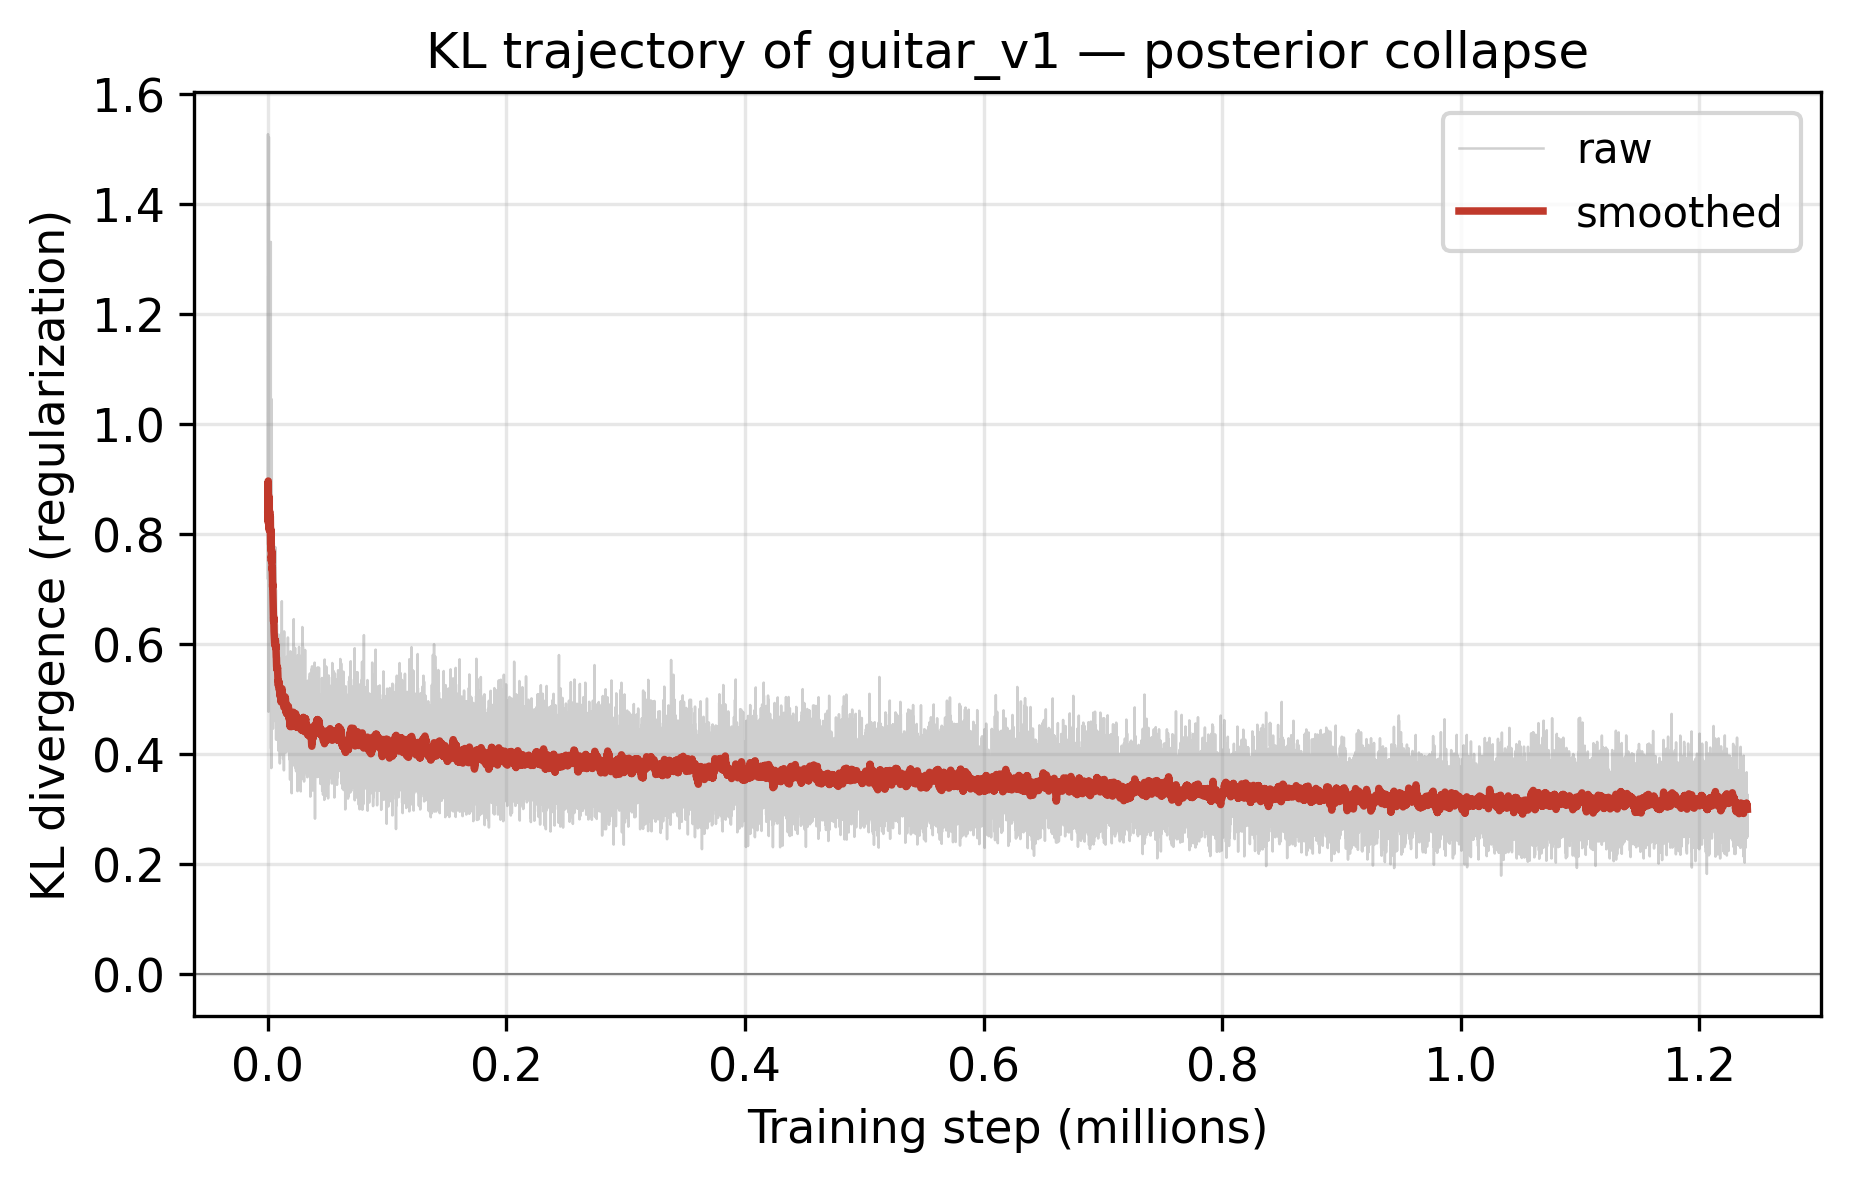
\includegraphics[width=0.85\textwidth]{../../figures/figure_5_1_guitar_v1_posterior_collapse.png}
\caption{KL divergence trajectory for guitar\_v1 during Phase~1 training. The KL term falls from approximately 0.83 at step zero to 0.25 by step 1.24\,M. A decreasing KL coupled with a decoder forward difference of 0.006 (below the 0.01 health threshold) constitutes the diagnostic signature of posterior collapse (mode~1 of the failure taxonomy, \S\ref{sec:failure_taxonomy}).}
\label{fig:kl_v1}
\end{figure}

In the next run (\texttt{guitar\_v2}) the $\beta$ warmup was applied and posterior collapse was no longer a problem. The model, however, did suffer a partial collapse because the latent space was too large. With \texttt{LATENT\_SIZE} of 128, the model achieved a utilisation of only approximately 0.005 nats per dimension. The diagnostics revealed a small encoder difference (0.79) and a decoder that was not reacting at all (forward difference $=0.003$). The output amplitude of 0.012 was roughly 60 times lower than the input signal. This implied that the 128-dimensional latent vector was too large for the $\sim$5.4-hour corpus available at that stage, and a reduction to 16 dimensions was therefore necessary.

\subsection{Iterations v3--v5: Adversarial Instabilities}\label{sec:guitar_v3v5}

The third and fourth iterations explored how dataset composition affected the model with the latent size reduced to 16. \texttt{guitar\_v3}, trained on 5.79 hours of mixed data, exhibited a partial response with forward differences peaking at 0.042. However, the model experienced Phase~2 generator collapse, meaning that the custom discriminator dominated the adversarial game.

\texttt{guitar\_v4} attempted to remedy this by using a cleaner, microphone-only dataset (3.05\,h compared to v3's 5.79\,h). Counter-intuitively, the reduction in data volume worsened the failure, leading to adversarial mode collapse. TensorBoard scalars revealed clear discriminator dominance: \texttt{pred\_real} reached 3.34 while \texttt{pred\_fake} fell to $-2.31$, producing a logit gap of 5.65 (Figure~\ref{fig:gan_gap_comparison}). Under these conditions the decoder produced a silence amplitude larger than the signal amplitude.

A focused experiment aimed at balancing the adversarial game was conducted in \texttt{guitar\_v5} by halving the discriminator's capacity. This produced the inverse failure: discriminator collapse. The \texttt{pred\_real} logit fell to $-0.90$, indicating that the discriminator was assigning negative scores to real audio, and the gap narrowed to 0.80. These findings, summarised in Table~\ref{tab:failure_summary}, indicated that no simple parameter scaling of the custom architecture could resolve the dominance/collapse axis.

\begin{figure}[H]
\centering
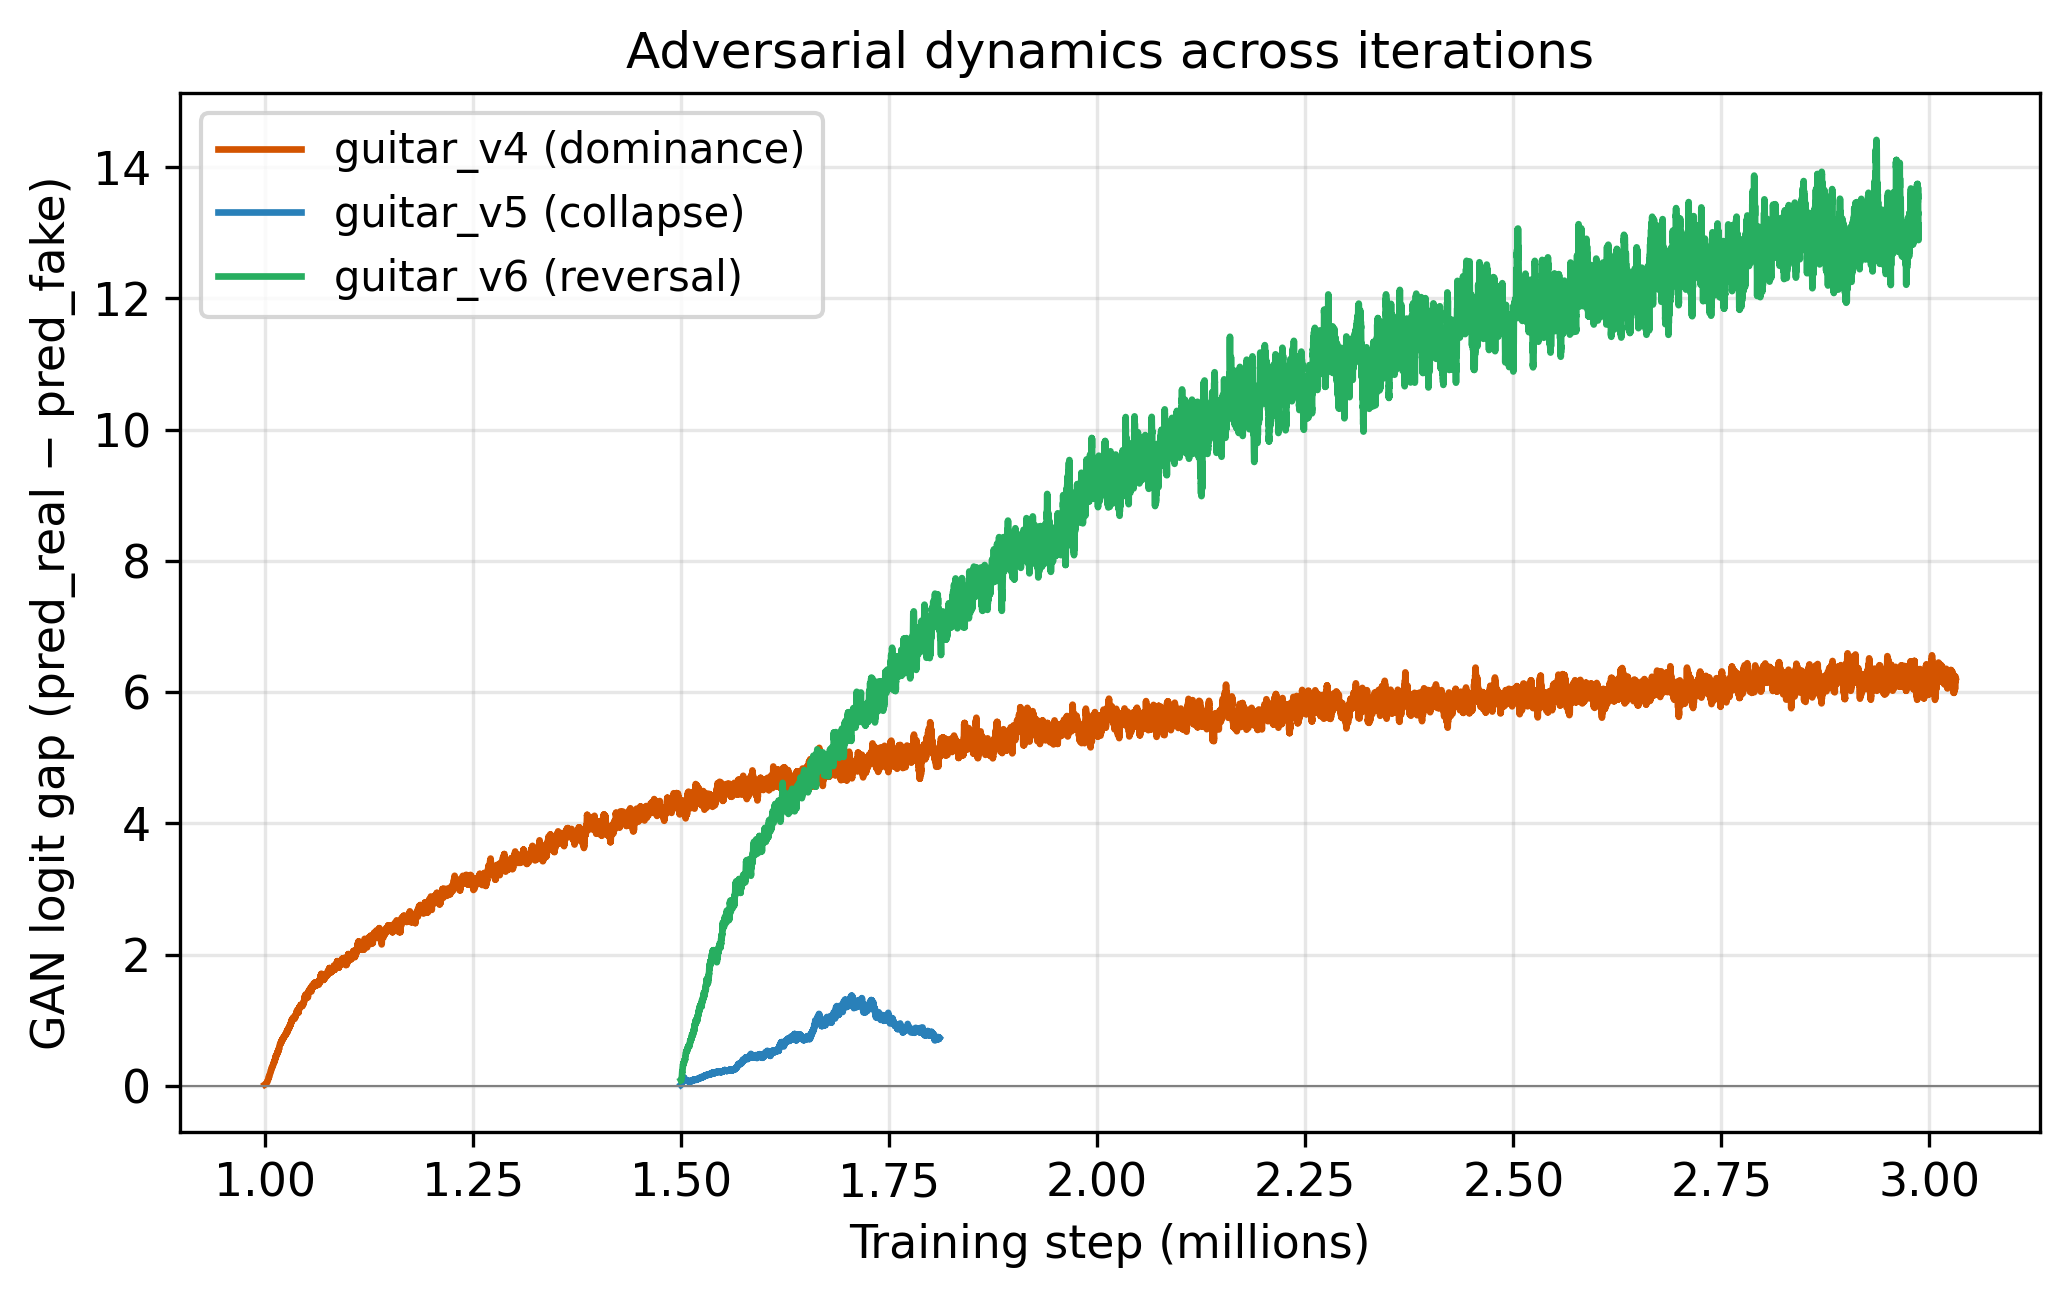
\includegraphics[width=0.95\textwidth]{../../figures/figure_5_2_gan_gap_comparison.png}
\caption{Adversarial dynamics across the three Phase-2 iterations: guitar\_v4 exhibits a widening GAN logit gap (peaks at 5.65, discriminator dominance); guitar\_v5 collapses to a narrow gap of approximately 0.80 (discriminator collapse); guitar\_v6 is the first checkpoint where the gap reverses direction during Phase~2, indicating an approximate adversarial equilibrium.}
\label{fig:gan_gap_comparison}
\end{figure}

\begin{table}[H]
\centering
\caption{Summary of failure modes across the guitar development iterations.}
\label{tab:failure_summary}
\footnotesize
\setlength{\tabcolsep}{5pt}
\begin{tabularx}{\textwidth}{@{}c>{\raggedright\arraybackslash}X>{\raggedright\arraybackslash}X>{\raggedright\arraybackslash}X@{}}
\toprule
\textbf{Iter.} & \textbf{Configuration} & \textbf{Failure mode} & \textbf{Diagnostic signature} \\
\midrule
v1 & Baseline \texttt{c128\_r10.gin} & Posterior collapse & KL falls $0.83\!\rightarrow\!0.25$; forward diff $0.006$ \\
v2 & $\beta$ warmup applied & Latent underutilisation & KL/dim $\approx 0.005$ nats; forward diff $0.003$ \\
v3 & \texttt{LATENT\_SIZE}$\rightarrow 16$ & Phase~2 collapse & Forward diff peaks at $0.042$ then degrades \\
v4 & Mic-only data ($3.05$\,h) & Adversarial mode collapse & Gap $=5.65$; silence amp.\ $>$ signal amp.\ \\
v5 & Halved discriminator & Discriminator collapse & \texttt{pred\_real}$=-0.90$; gap $=0.80$ \\
v6 & Official RAVE v2 base & Working in-distribution autoencoder & STFT corr.\ calibrated in Table~\ref{tab:stft_calibration}; GAN-gap reversal \\
\bottomrule
\end{tabularx}
\end{table}

\subsection{Iteration v6: Working Autoencoder}\label{sec:guitar_v6}

The final iteration (\texttt{guitar\_v6}) was based on the RAVE v2 official architecture and \texttt{causal.gin} overrides. In Phase~2 the GAN logit gap was observed to reverse for the first time in the series, suggesting that an adversarial equilibrium had been reached. Listening tests indicated perceptually recognisable reconstruction of in-distribution guitar audio at epoch 1935 (mid-Phase-2), and this checkpoint was therefore selected as canonical. The final epoch (2511) showed slightly degraded performance under the same listening criteria. Under the operational diagnostic of \S\ref{sec:diagnostic_method}, output amplitude rose from the near-silent levels of the collapsed checkpoints v1--v3 (output RMS $\approx 0.003$--$0.005$) to RMS $\approx 0.024$ on the canonical guitar\_v6 checkpoint and 0.041 on the Phase~1 reconstruction-only state, which together suggest a meaningful recovery of decoder responsiveness.

A quantitative reconstruction test on the canonical checkpoint, using eight GuitarSet solo-microphone samples of five seconds each (STFT parameters: \texttt{n\_fft}$=2048$, hop$=512$), yielded a mean STFT magnitude correlation of 0.16 (0.17 with time-shift alignment). This value falls below the 0.3 heuristic proposed initially in \S\ref{sec:diagnostic_method}. To understand whether this gap reflects a limitation of the model or of the metric, the same evaluation was applied to every preceding checkpoint in the iteration sequence; the results are reported in \S\ref{sec:stft_calibration}. Anticipating the finding of that calibration: the STFT magnitude correlation does not differentiate working from collapsed checkpoints in the expected direction, and the operational evaluation of guitar\_v6 as a working in-distribution autoencoder therefore rests on the combined evidence of (i)~listening tests, (ii)~output amplitude recovery, and (iii)~Phase~2 GAN gap reversal.

\begin{figure}[H]
\centering
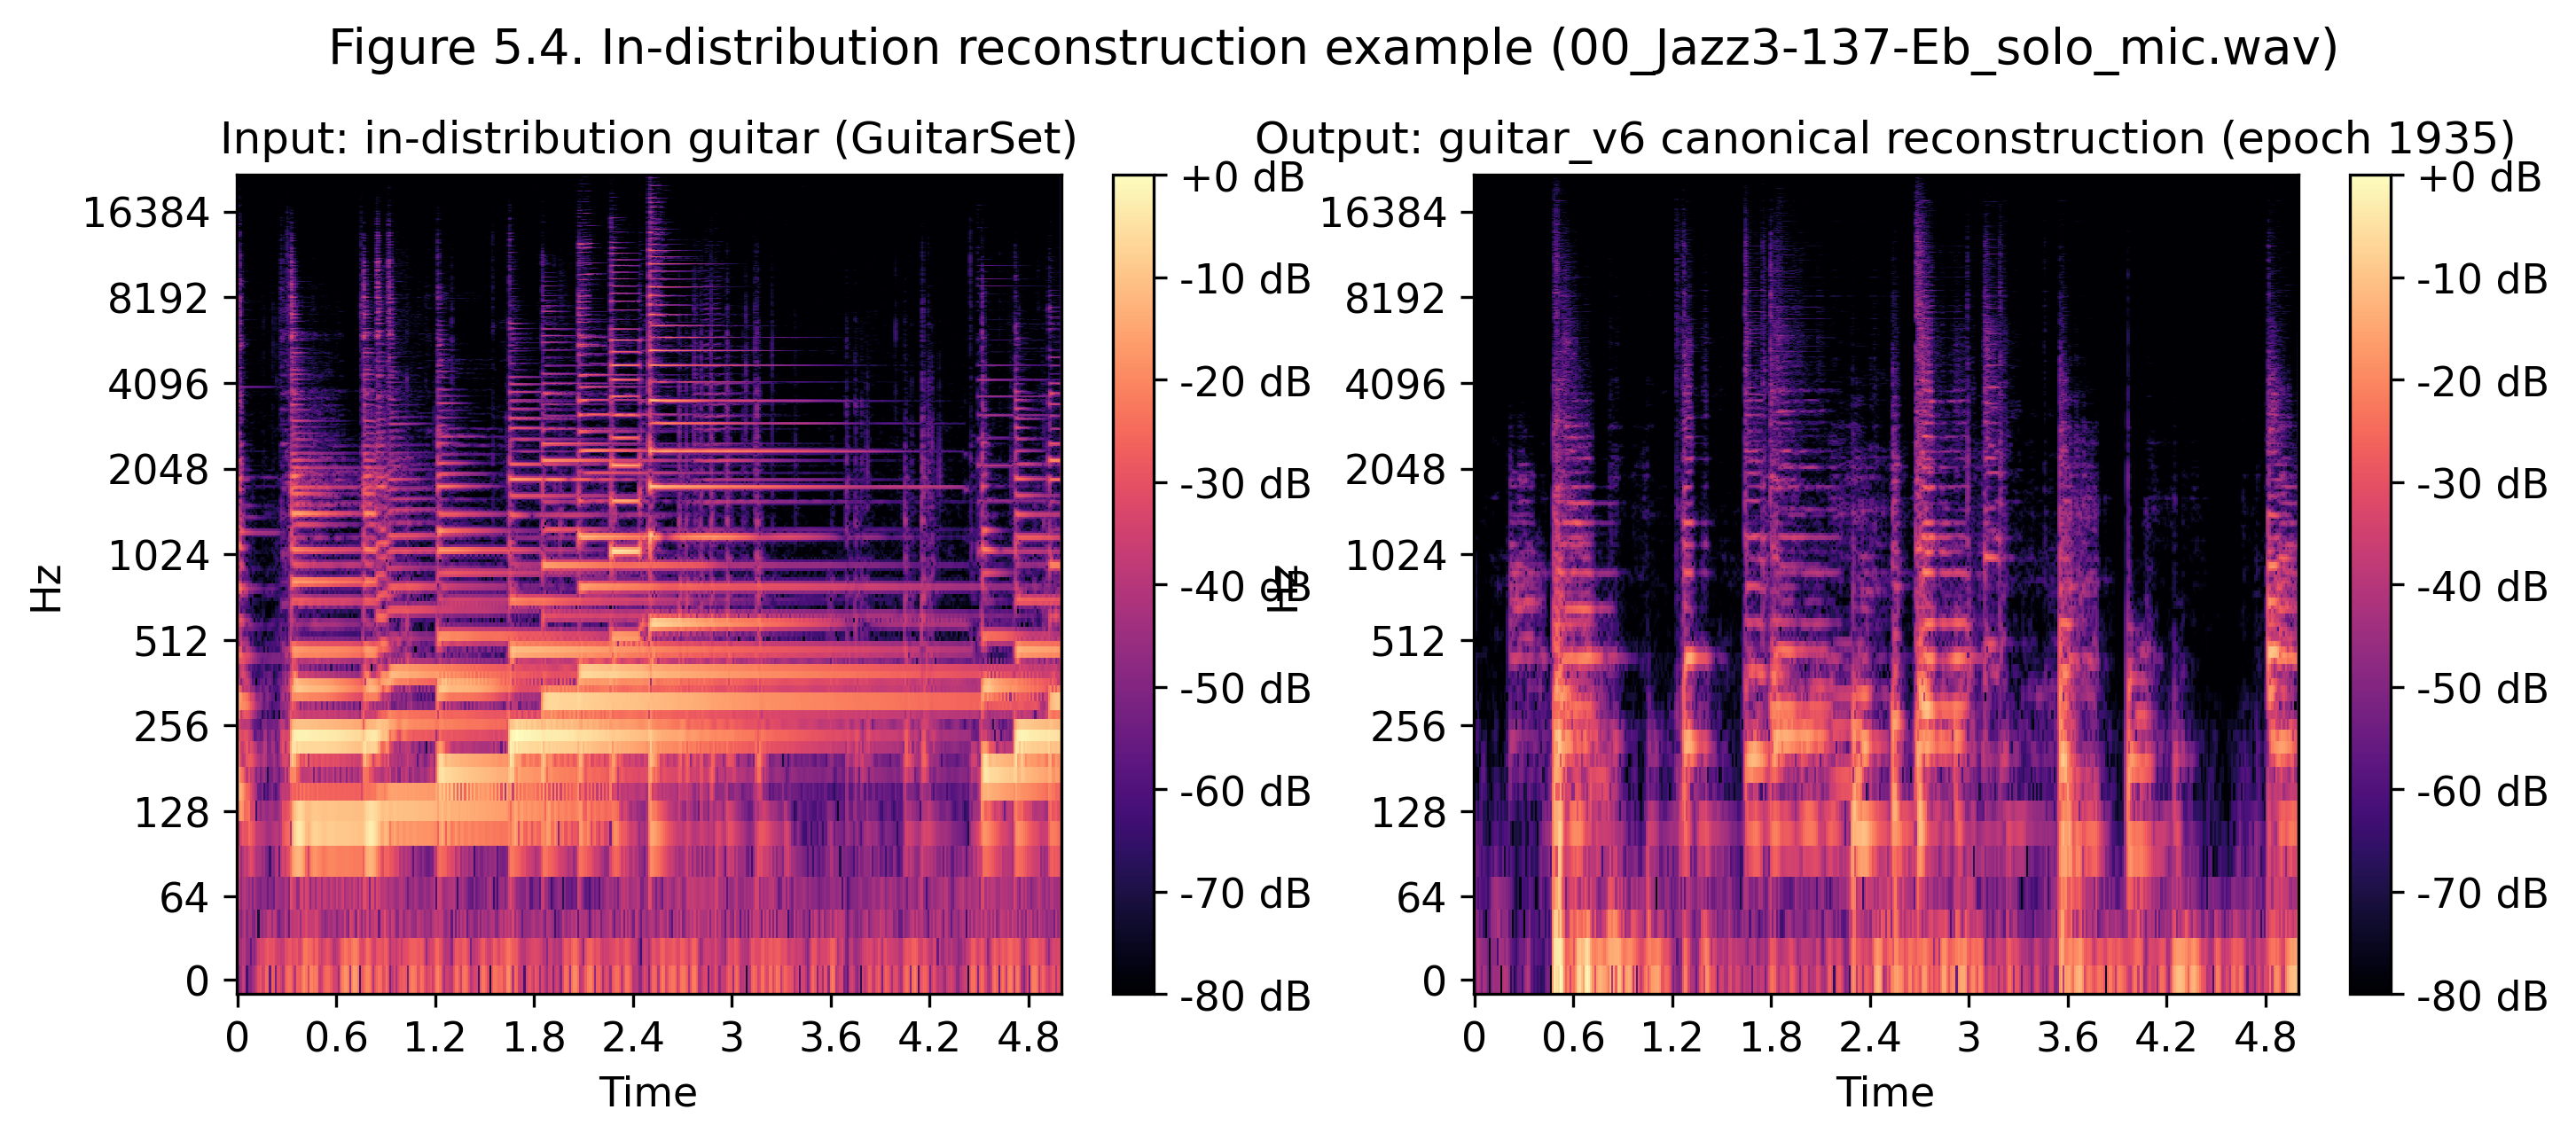
\includegraphics[width=0.95\textwidth]{../../figures/figure_5_4_spectrogram_in_dist.png}
\caption{STFT magnitude spectrograms (log scale) for an in-distribution GuitarSet sample: input (left) and the canonical guitar\_v6 reconstruction (right). The reconstructed spectrogram preserves the harmonic structure and onset patterns of the input although it lacks fine spectral detail above approximately 4\,kHz.}
\label{fig:spectrogram_in_dist}
\end{figure}

The same in-distribution success did not transfer to voice input, which is out-of-distribution (OOD) for the trained model. The encoder was capable of differentiating the vocal signals --- latent differences between distinct vocal inputs ranged from 1.27 to 6.89 --- but the decoder produced a practically uniform, low-energy output. This suggests that the encoder can map voice into latent space, but the resulting trajectories lie outside the trained guitar manifold, and the decoder lacks the generative coverage required to render them.

\subsection{Calibration of the STFT-Magnitude-Correlation Diagnostic}\label{sec:stft_calibration}

To assess whether the STFT magnitude correlation criterion of \S\ref{sec:diagnostic_method} robustly discriminates working autoencoders from collapsed ones, the same in-distribution reconstruction test was applied to every checkpoint in the iteration sequence. Eight GuitarSet solo-microphone samples of five seconds each were evaluated against each checkpoint with identical STFT parameters (\texttt{n\_fft}$=2048$, hop$=512$). Results are summarised in Table~\ref{tab:stft_calibration}.

\begin{table}[H]
\centering
\caption{Cross-checkpoint calibration of the STFT-magnitude-correlation diagnostic. All values are means across $N=8$ GuitarSet samples. Output RMS reflects the energy of the model output relative to the input (mean input RMS $\approx 0.065$).}
\label{tab:stft_calibration}
\footnotesize
\setlength{\tabcolsep}{6pt}
\begin{tabularx}{\textwidth}{@{}>{\raggedright\arraybackslash}p{4.6cm}>{\raggedright\arraybackslash}XS[table-format=1.3]S[table-format=1.2]S[table-format=1.2]@{}}
\toprule
\textbf{Checkpoint} & \textbf{Diagnostic state} & {\textbf{Output RMS}} & {\textbf{STFT (raw)}} & {\textbf{STFT (aligned)}} \\
\midrule
guitar\_v1 & Posterior collapse & 0.005 & 0.16 & 0.16 \\
guitar\_v2 & Latent underutilisation & 0.003 & 0.24 & 0.25 \\
guitar\_v3 & Phase~2 generator collapse & 0.004 & 0.24 & 0.26 \\
guitar\_v4 & Adversarial mode collapse & 0.021 & 0.25 & 0.26 \\
guitar\_v5 & Discriminator collapse & 0.024 & 0.26 & 0.28 \\
guitar\_v6 Phase 1 (ep.\ 1499) & Reconstruction-only & 0.041 & 0.19 & 0.21 \\
\textbf{guitar\_v6 best (ep.\ 1935)} & \textbf{Working autoencoder (canonical)} & \textbf{0.024} & \textbf{0.16} & \textbf{0.17} \\
guitar\_v6 final (ep.\ 2511) & Working, slightly degraded & 0.024 & 0.14 & 0.17 \\
\bottomrule
\end{tabularx}
\end{table}

Two observations follow from Table~\ref{tab:stft_calibration}. First, no checkpoint reaches the 0.3 heuristic that was proposed initially in \S\ref{sec:diagnostic_method} as the threshold for ``perceptually acceptable'' reconstruction; the maximum observed value across all checkpoints is 0.28 (time-aligned, guitar\_v5). Second, and more revealing, the STFT magnitude correlation does not differentiate between working autoencoders and known-collapsed checkpoints in the expected direction: collapsed checkpoints v2--v5 score equal to or slightly higher than the working guitar\_v6 canonical checkpoint.

The reason is structural rather than incidental. Collapsed checkpoints produce near-silent outputs (RMS $\approx 0.003$--$0.024$ versus input RMS $\approx 0.065$); the STFT magnitudes of such outputs are uniformly small but nonetheless share the general spectral envelope of any natural audio source (low-frequency dominance, high-frequency attenuation). The flattened Pearson correlation between this trivial envelope and the input's STFT therefore captures shared spectral shape rather than genuine reconstruction. Output RMS, by contrast, does discriminate: collapsed checkpoints produce outputs an order of magnitude quieter than the working autoencoder's Phase~1 reconstruction-only state (guitar\_v6 Phase~1, RMS $=0.041$).

This finding constitutes a calibration limitation of the diagnostic methodology defined in \S\ref{sec:diagnostic_method}. The STFT magnitude correlation criterion was empirically derived from preliminary comparisons but was not stress-tested against the full iteration sequence at the time of definition. The full calibration in Table~\ref{tab:stft_calibration} reveals that the metric was insufficient as a sole discriminator; output amplitude and informal listening evaluation were therefore retained as the operational evaluators for canonical-checkpoint selection (\S\ref{sec:guitar_v6}). The threshold of 0.3 should be understood as a working initial proposal rather than a validated criterion; future replication studies on this diagnostic framework should re-derive the threshold using outputs from both working and collapsed reference models in the target setup.

\section{Drums}\label{sec:drums}

The drum-kit evaluation aimed to apply the BRAVE streaming-causal recipe of \textcite{caspe2025brave} to the 10.86-hour Groove corpus.

The initial drum iteration (\texttt{drums\_v1}), using the \texttt{c16\_r10\_beta\_fixed.gin} configuration, resulted in a forward difference of 0.0045. This was below the 0.01 threshold defined for tonal responsiveness. Initial informal listening tests suggested that voice consonants and beatbox transients gave rise to recognisable drum-like timbres in Pure Data, although subsequent re-listening at a later date with the same test setup did not reproduce a perceptually compelling voice-to-drum mapping. The numerical diagnostic indicates that a ``working voice-to-drums'' claim cannot be substantiated on spectral evidence alone.

The second iteration (\texttt{drums\_v2}) applied the configuration template established in \texttt{guitar\_v6} (the official \texttt{v2.gin} architectural baseline with the project's \texttt{causal} overrides) to the Groove corpus and was trained for approximately 95 hours ($\approx 2.28$\,M steps). Phase~1 concluded with healthy validation scores (\texttt{val} $\approx 4.1$, \texttt{mb\_spec} $\approx 3.7$). However, Phase~2 exhibited a monotonic widening of the GAN gap from 9.8 to 20.3 over 800,000 steps (Figure~\ref{fig:drums_v2_gan}), while the validation loss plateaued around 7.5. Training was terminated before the scheduled time as discriminator dominance reproduced despite the \texttt{update\_discriminator\_every=4} safeguard provided by the v2 architecture. This indicates that the \texttt{guitar\_v6} configuration template did not transfer cleanly from the guitar dataset to the drum dataset under these specific training constraints.

\begin{figure}[H]
\centering
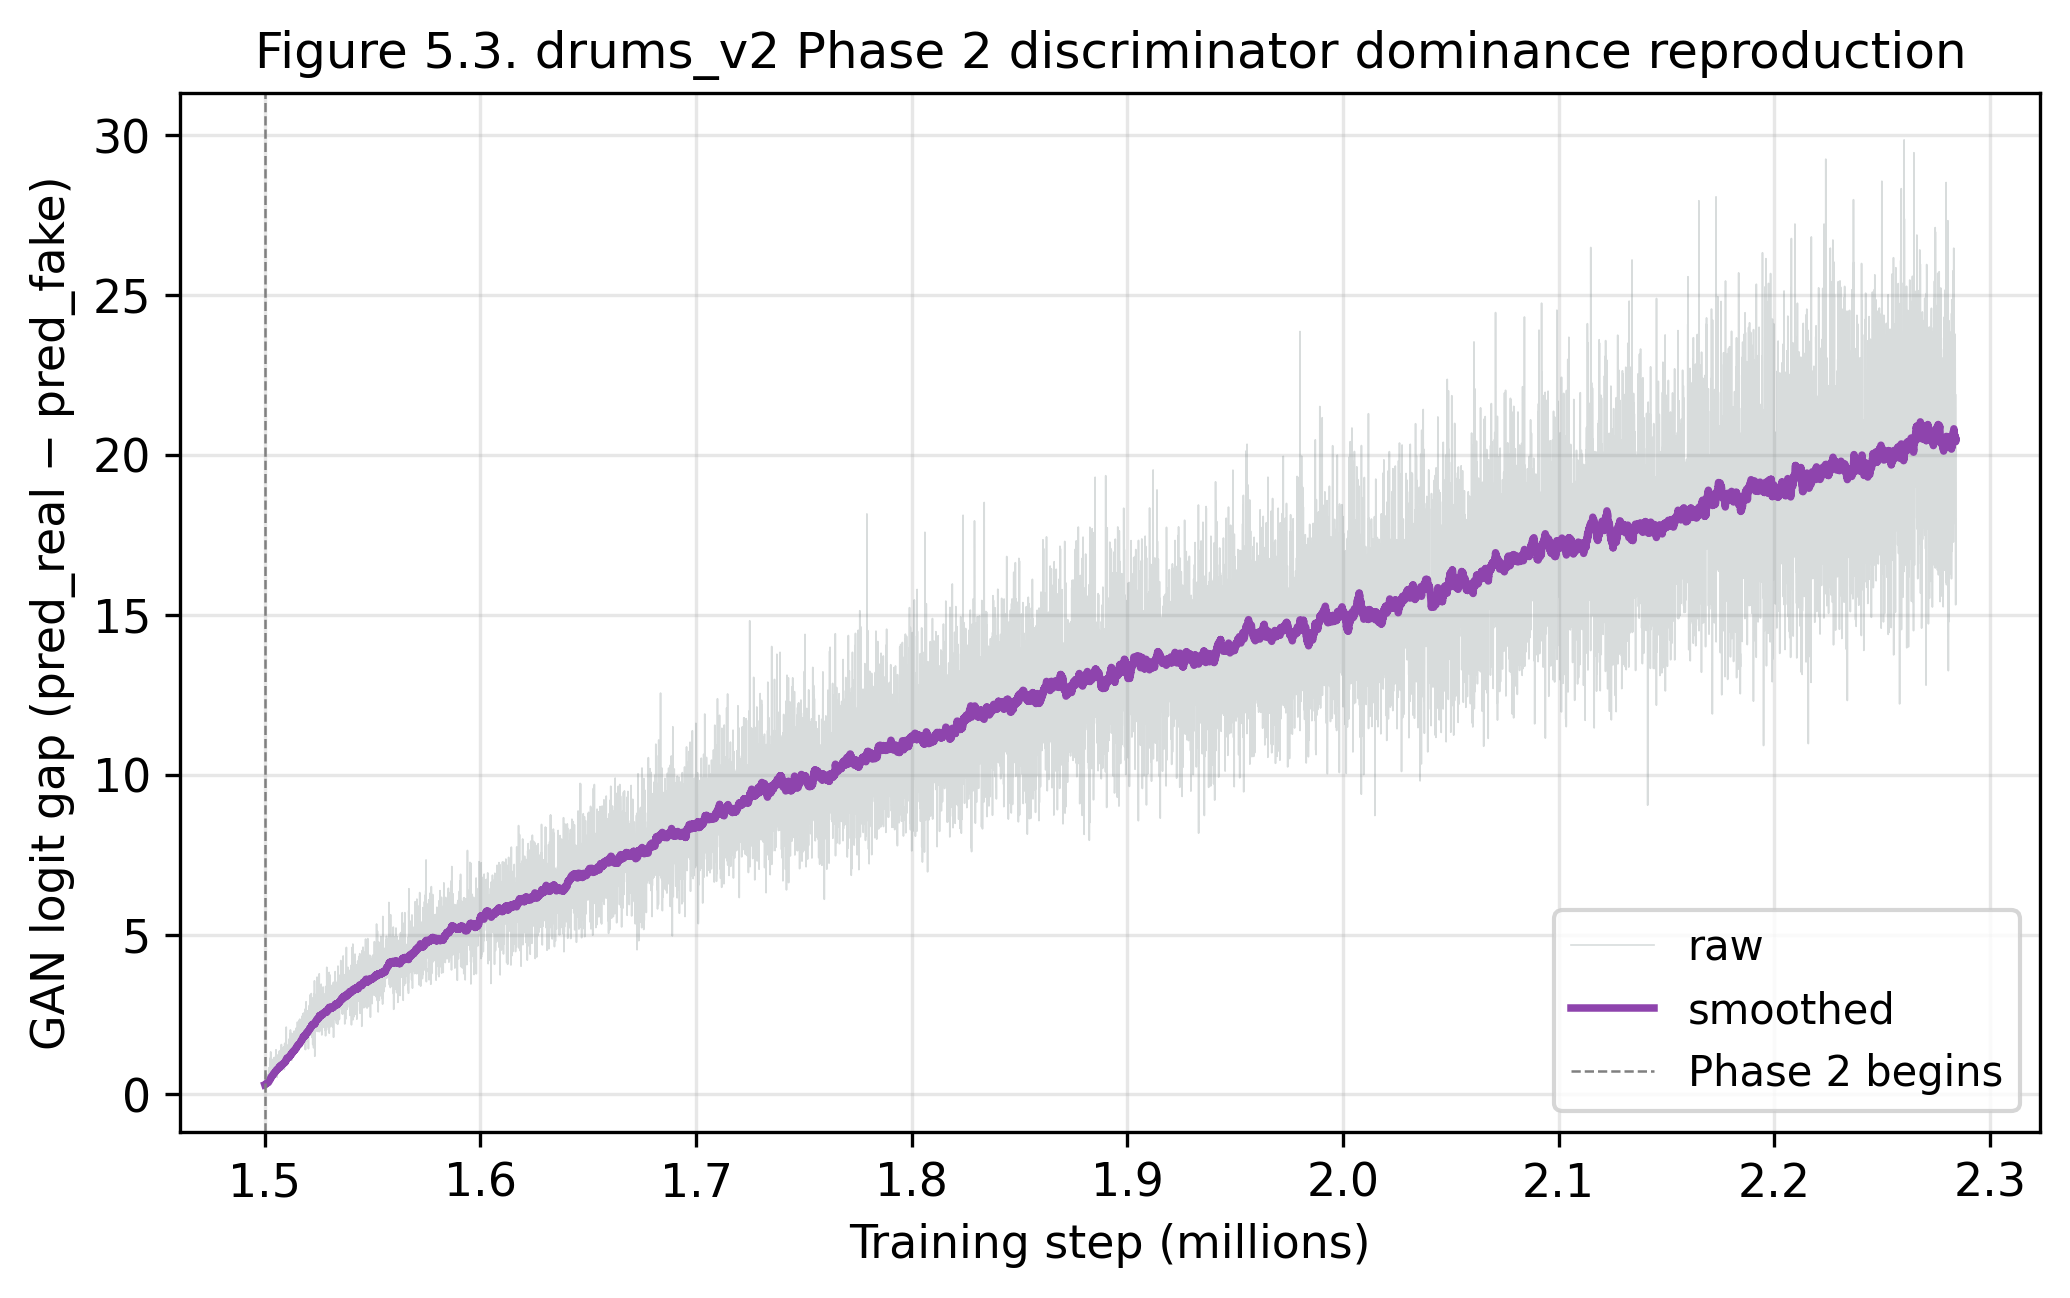
\includegraphics[width=0.95\textwidth]{../../figures/figure_5_3_drums_v2_gan_widening.png}
\caption{drums\_v2 GAN logit gap over the duration of training. Phase~1 (steps 0--1.5\,M) maintains a near-zero adversarial gap. From Phase~2 onset onward, the gap widens monotonically from approximately 9.8 to over 20, reproducing the discriminator-dominance pattern previously observed in guitar\_v3/v4 despite the use of \texttt{update\_discriminator\_every=4}.}
\label{fig:drums_v2_gan}
\end{figure}

\section{External Baseline: IRCAM Percussion}\label{sec:ircam_baseline}

To determine whether the OOD limitations observed in iterations v6 and \texttt{drums\_v1} were inherent to the BRAVE architecture, a comparative diagnostic was performed using the official ACIDS-IRCAM percussion model (71\,MB TorchScript) \parencite{acidsircam2024models}. When subjected to the same synthetic-input test described in \S\ref{sec:diagnostic_method}, the IRCAM model yielded a forward difference (silence vs.~noise) of 1.75. This indicates that the official model is more responsive than the \texttt{drums\_v1} iteration (forward difference 0.0045) by more than two orders of magnitude under this diagnostic.

The IRCAM model respected silence (0.001 output for silent input) and, in informal Pure Data listening tests with voice input, produced audibly modulated percussive output. This indicates that a well-trained BRAVE model with higher-quality or more voluminous data can overcome the manifold-mapping bottleneck. This comparison supports the conclusion that the performance-limiting factors of the present models are training recipe and data scale rather than fundamental architectural constraints of BRAVE.

\subsection{Candidate Explanations for the IRCAM Responsiveness Gap}\label{sec:ircam_hypothesis}

The IRCAM percussion baseline being more responsive than \texttt{drums\_v1} by more than two orders of magnitude on the same diagnostic raises the question of what specifically in IRCAM's training recipe accounts for the gap. The official model was not accompanied by a training-protocol publication at the time of writing, so the candidates below are framed as informed hypotheses grounded in the broader RAVE/BRAVE literature rather than as established findings. Each is identified as a candidate for empirical follow-up in \S\ref{sec:future_work}.

\paragraph{Hypothesis 1 --- Training data scale.} The published RAVE training compendium recommends a minimum of three hours of in-distribution audio and suggests that significantly larger corpora (tens of hours upward) produce more robust models. Although the present drums corpus (Groove MIDI Dataset, $\approx 10.86$\,h) satisfies the recommended minimum, it is plausible that the IRCAM percussion model was trained on a larger corpus collected from multiple percussion sources. Larger datasets are known empirically to mitigate the discriminator-dominance pattern that terminated drums\_v2 (\S\ref{sec:drums}).

\paragraph{Hypothesis 2 --- Dataset homogeneity.} Our consolidated guitar corpus exhibited a 35.9\,dB noise-floor spread across recording paths (\S\ref{sec:noise_floor}), which the encoder is well positioned to encode as a salient latent feature at the expense of timbral discrimination. Although the drums corpus did not undergo the same per-source analysis, the Groove MIDI Dataset combines multiple drummers and kit configurations. Curated single-source corpora --- which IRCAM-quality pretrained models are typically trained on --- avoid this heterogeneity penalty.

\paragraph{Hypothesis 3 --- Architectural variant (RAVE v3 with AdaIN).} Recent ACIDS-IRCAM releases have incorporated the RAVE v3 architecture, which adds Snake activations, a Descript-style discriminator, and Adaptive Instance Normalisation (AdaIN) for explicit cross-domain style transfer. AdaIN in particular is designed to bridge timbre gaps between source and target domains in a way that v1 and v2 architectures are not. If the IRCAM percussion checkpoint was produced with a v3 configuration --- which we cannot determine without access to its training metadata --- the responsiveness to OOD voice input would not be surprising. The 32\,GB VRAM requirement of v3 prevented us from testing this hypothesis directly on the present 16\,GB GPU.

\paragraph{Hypothesis 4 --- Training duration and Phase~2 schedule.} Our iterations targeted approximately 3\,M total steps with a Phase~1 of 1.5\,M for v6 and drums\_v2. Several community-reported recipes extend Phase~2 beyond 3\,M steps before declaring training complete, particularly for percussion datasets where transient quality is dominated by adversarial fine-tuning rather than spectral reconstruction. The drums\_v2 trajectory was terminated at 2.28\,M (mid-Phase-2) for resource reasons; it is open whether further training would have stabilised or aggravated the dominance pattern.

\paragraph{Hypothesis 5 --- Augmentation.} The acids-rave 2.3.1 training pipeline exposes \texttt{--augment gain --augment mute} flags, but in our setup these are non-operational: \texttt{compress} and \texttt{RandomCompress} depend on \texttt{torchaudio.sox\_effects} which is removed in current torchaudio releases, and inspection of the upstream \texttt{RandomGain} transform shows a bug whereby the gain-adjusted signal \texttt{x\_amp} is computed but the original \texttt{x} is returned. Reference IRCAM training pipelines may use augmentation either through patched versions of the same library or through external preprocessing; this would teach the encoder amplitude- and silence-invariance that our trained encoder lacks.

Disentangling these candidates would require either access to the IRCAM training metadata or a controlled replication study varying one factor at a time on our infrastructure. Both are identified as priorities for the future work outlined in \S\ref{sec:future_work}.

\section{Failure-Mode Taxonomy}\label{sec:failure_taxonomy}

The outcomes of the iterative training campaign can be summarised into five chief failure modes relevant to streaming VAE resynthesis. These modes, discovered through the Python diagnostics described in Chapter~\ref{chap:implementation}, serve as guides to the stabilisation of similar real-time models.

\begin{enumerate}
\item \textbf{Posterior collapse (v1).} Identifiable by a falling KL trajectory and a decoder that ignores the latent space. Caused by applying KL pressure before reconstruction has been learned.
\item \textbf{Latent underutilisation (v2).} Identifiable by very low nats-per-dimension ($\approx 0.005$) and a near-silent decoder. Occurs when the bottleneck capacity exceeds the dataset's information density.
\item \textbf{Discriminator dominance / generator mode collapse (v3, v4, drums\_v2).} Marked by a widening discriminator logit gap (typically $>5$) and, in the worst case, silence amplitude exceeding signal amplitude. Triggered when the default custom discriminator out-paces the generator during Phase~2.
\item \textbf{Discriminator collapse (v5).} The inverse failure --- heuristic discriminator weakening pushed \texttt{pred\_real} to negative values and narrowed the logit gap to 0.80. Confirmed that no simple capacity-scaling resolves the dominance/collapse axis.
\item \textbf{OOD decoder behaviour (v6, drums\_v1).} A structural failure where the encoder differentiates non-instrument input (e.g.\ voice), but the decoder fails to render it because the resulting latent coordinates reside outside the trained manifold.
\end{enumerate}

As the IRCAM baseline comparison (\S\ref{sec:ircam_baseline}, \S\ref{sec:ircam_hypothesis}) confirms, these should be regarded as training-recipe failures rather than architectural limitations of BRAVE. Addressing them in future work will require more homogeneous datasets and possibly explicit pitch-conditioning to close the cross-modal gap.

\section{Noise-Floor Heterogeneity in the Guitar Corpus}\label{sec:noise_floor}

Chapter~\ref{chap:methodology}, \S\ref{sec:datasets_preprocessing} introduced the heterogeneity concern that arises from combining recordings captured through different paths into a single training corpus. To characterise that heterogeneity quantitatively, the noise-floor methodology defined in \S\ref{sec:datasets_preprocessing} was applied to every source recording of the consolidated guitar corpus (919 files across six recording paths). For each file, the Root Mean Square energy was computed in non-overlapping 100\,ms windows; the 5th percentile of these RMS values was taken as the noise-floor estimate and converted to dBFS. Per-source aggregates are reported in Table~\ref{tab:noise_floor} and visualised in Figure~\ref{fig:noise_floor}. The analysis was performed on the source recordings; the 52 Guitar-TECHS files measured here were reduced to 32 in the final training corpus of Table~\ref{tab:guitar_corpus} (899 files in total) after 20 stereo files were removed during the mono-conversion stage, so the two totals differ only by that filtering step.

\begin{table}[H]
\centering
\caption{Per-source noise-floor distribution across the source recordings of the consolidated guitar corpus (919 files; see text for the relationship to the 899-file training corpus of Table~\ref{tab:guitar_corpus}). The 5th-percentile RMS in 100\,ms windows estimates the noise floor of each recording.}
\label{tab:noise_floor}
\begin{tabular}{lcccc}
\toprule
\textbf{Source} & \textbf{\textit{n} files} & \textbf{Recording method} & \textbf{Noise floor (dBFS, median)} & \textbf{IQR (dB)} \\
\midrule
GuitarSet & 360 & Mic-captured acoustic & $-46.5$ & 10.4 \\
Guitar-TECHS & 52 & Electric direct input & $-67.2$ & 28.1 \\
IDMT acoustic\_mic & 128 & Mic-captured acoustic & $-57.8$ & 7.1 \\
IDMT acoustic\_pickup & 128 & Pickup capture & $-53.3$ & 9.4 \\
IDMT Career SG & 123 & Electric direct input & $\mathbf{-82.4}$ & 7.2 \\
IDMT Ibanez 2820 & 128 & Electric direct input & $-71.5$ & 11.3 \\
\bottomrule
\end{tabular}
\end{table}

\begin{figure}[H]
\centering
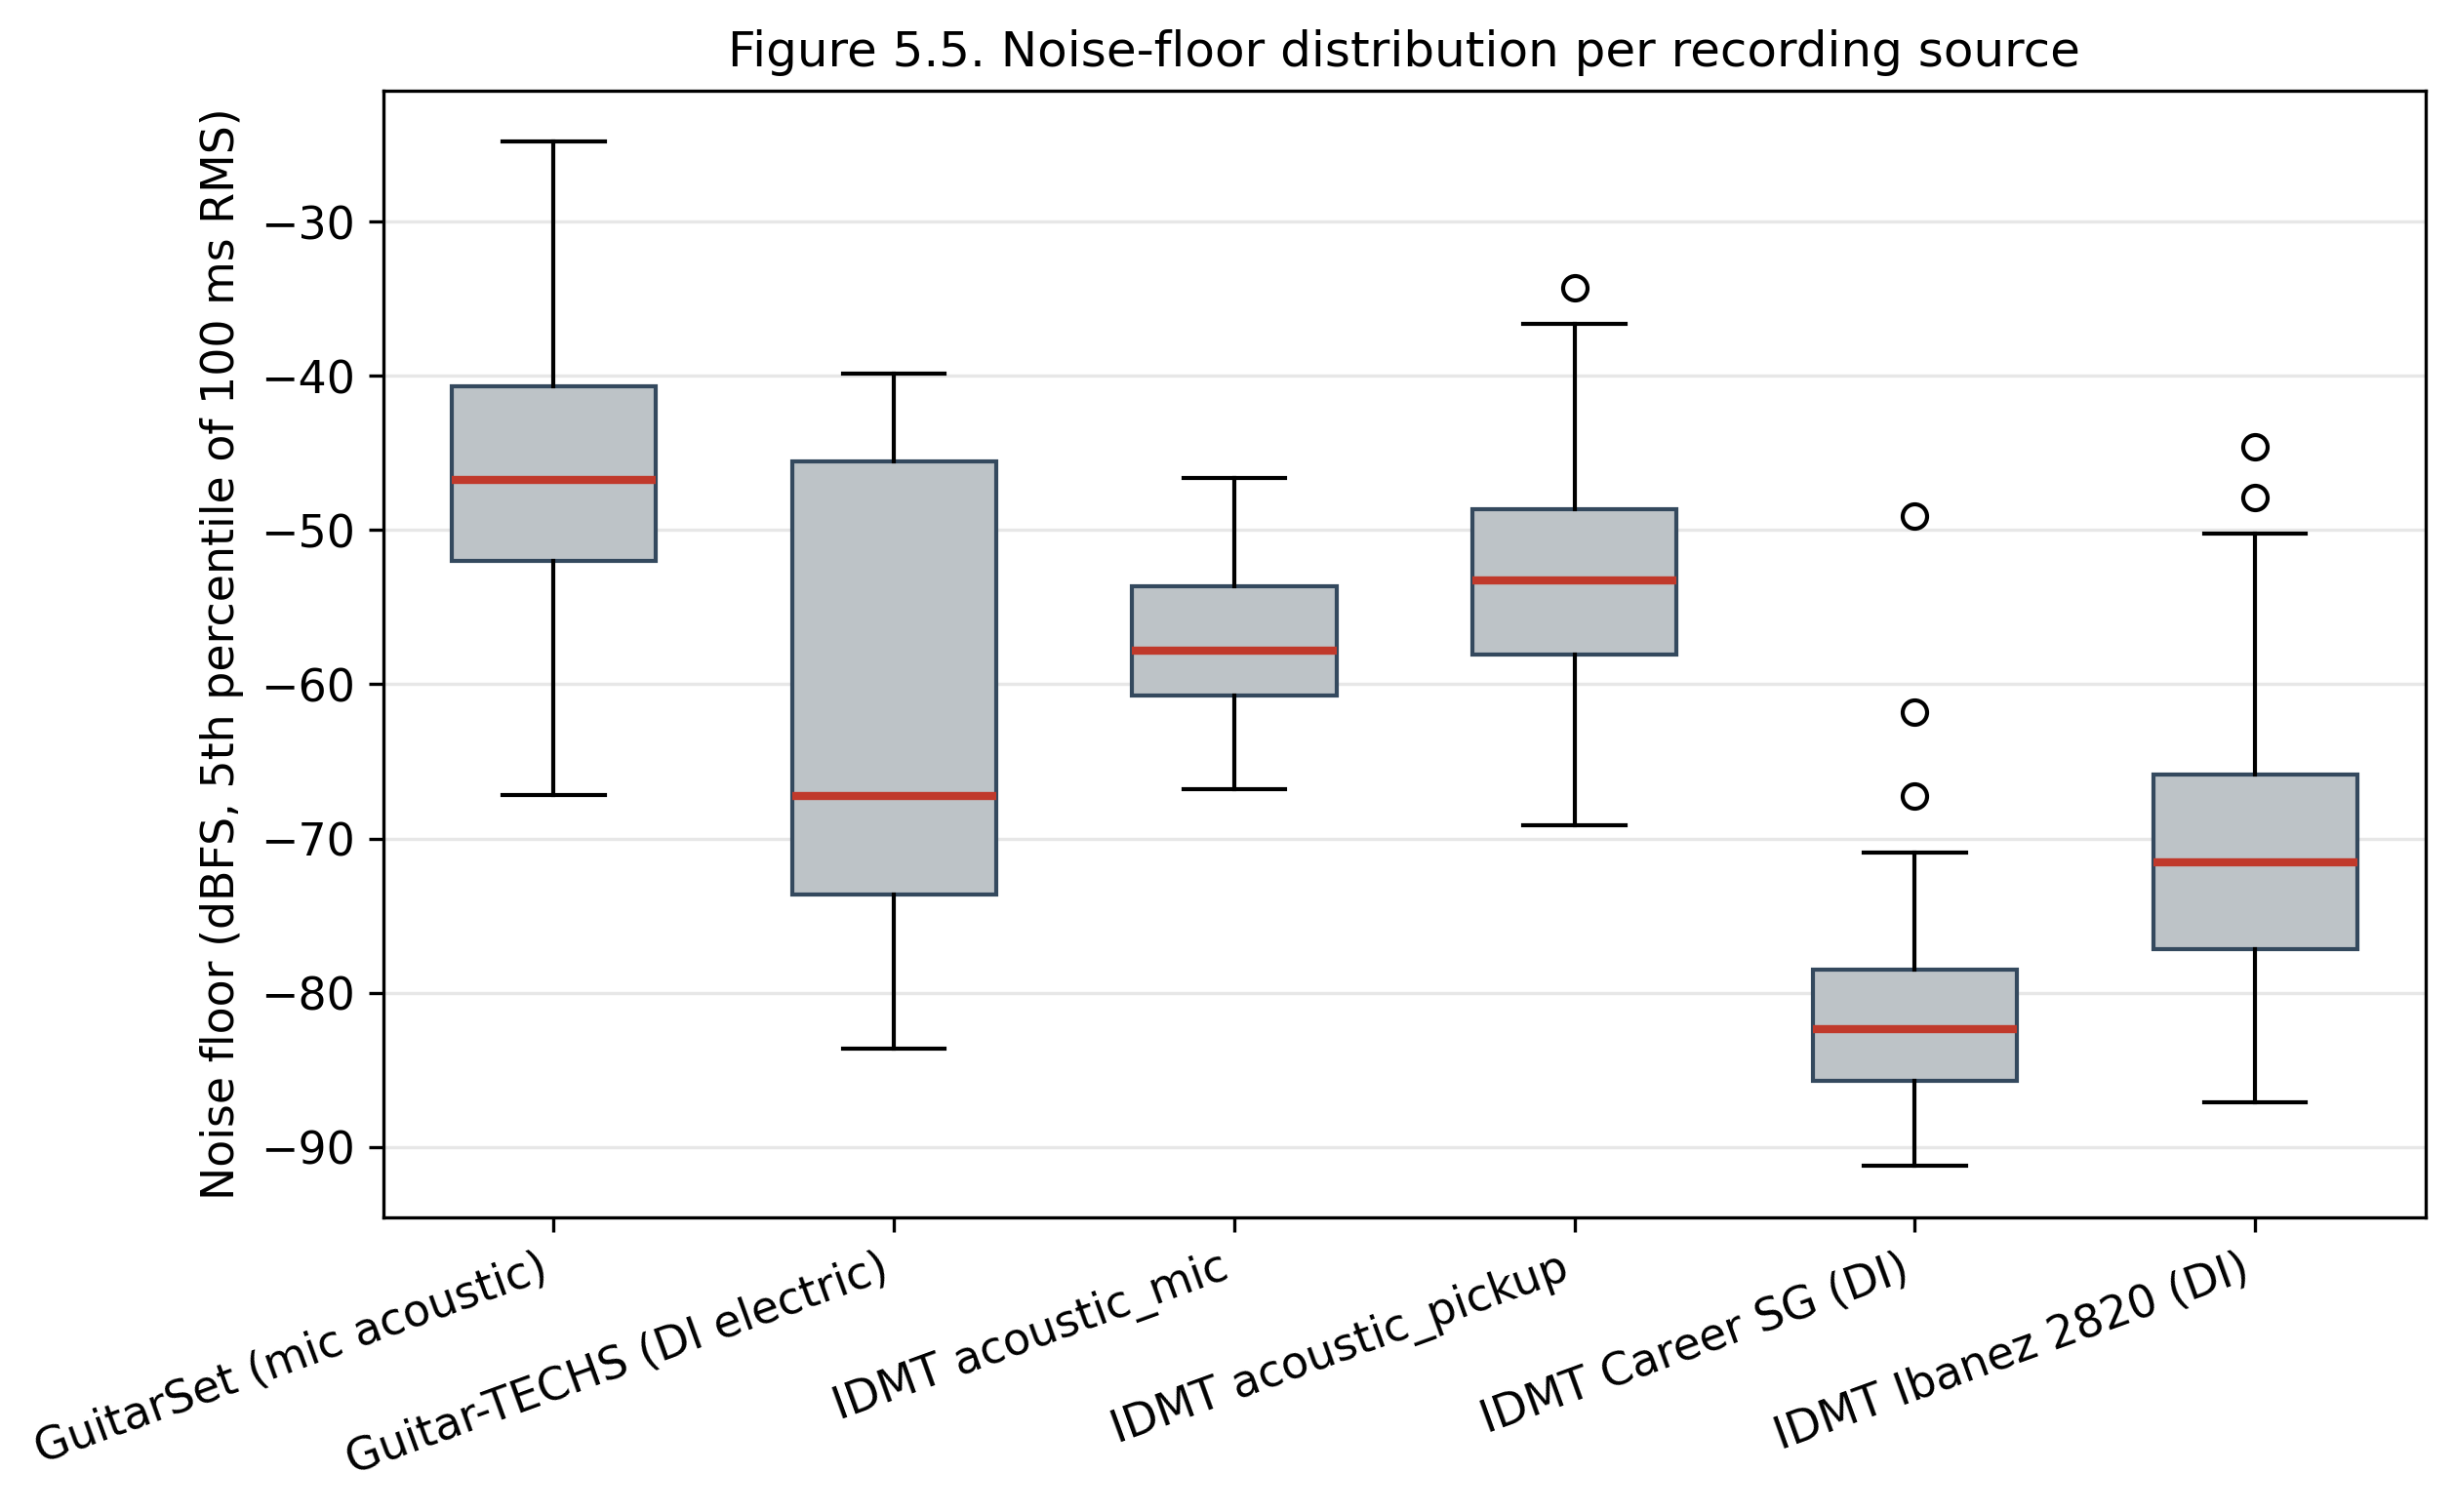
\includegraphics[width=0.95\textwidth]{../../figures/figure_5_5_noise_floor.png}
\caption{Per-source noise-floor distribution across the source recordings of the consolidated guitar corpus (boxplots; $n=360, 52, 128, 128, 123, 128$ files respectively). Median noise floors range from $-82.4$\,dBFS (IDMT Career SG DI) to $-46.5$\,dBFS (GuitarSet mic-captured acoustic), a 35.9\,dB spread that exceeds typical within-performance dynamic variation.}
\label{fig:noise_floor}
\end{figure}

The spread between the cleanest source (IDMT Career SG direct input, median $-82.4$\,dBFS) and the loudest source (GuitarSet mic-captured acoustic, median $-46.5$\,dBFS) is 35.9\,dB. To contextualise that figure, the typical dynamic variation within a single guitar performance is approximately 20--30\,dB between \textit{pianissimo} and \textit{fortissimo} passages, so the inter-source noise-floor spread exceeds the within-performance dynamic range by an order of magnitude.

A consequence anticipated in \S\ref{sec:datasets_preprocessing} is that the encoder may treat the recording method as a salient latent feature, allocating capacity to discriminate among capture paths rather than among timbral characteristics. The present study did not directly test this hypothesis through a controlled latent-clustering experiment; this is identified as a candidate analysis for future work (\S\ref{sec:future_work}). However, the magnitude of the per-source spread reported here provides quantitative grounding for the limitation acknowledged throughout the thesis: the combined corpus, although it satisfies RAVE's recommended duration window \parencite{caillon2021rave}, is heterogeneous on a dimension that the model is well positioned to encode.

Two practical implications follow. First, the iteration sequence's reliance on the combined corpus from v3 onwards (after the smaller v1/v2 single-source corpus failed to support a 128-dimensional latent) made dataset homogeneity a secondary priority to dataset scale, a trade-off discussed in \S\ref{sec:datasets_preprocessing} and revisited in \S\ref{sec:future_work}. Second, the contrast with the IRCAM percussion baseline (\S\ref{sec:ircam_baseline}) --- trained on a presumably more curated corpus --- supports the conclusion that training-recipe choices including corpus selection rather than BRAVE architecture per se account for the responsiveness gap.

% ============================================================================
%  CHAPTER 6 -- CONCLUSIONS AND FUTURE WORK
% ============================================================================
\chapter{Conclusions and Future Work}\label{chap:conclusions}

\section{Summary of Findings}\label{sec:summary_findings}

This thesis explored the feasibility of the streaming-causal BRAVE architecture for voice-driven instrument resynthesis with less than 10\,ms latency when trained on heterogeneous, limited-scale datasets. The study went through six versions of the guitar model (v1--v6) and two versions of drums (\texttt{drums\_v1}, \texttt{drums\_v2}). It was found that \texttt{guitar\_v6}, which used the official \texttt{v2.gin} and \texttt{causal.gin} configurations along with a smaller latent size of 16 and a longer Phase~1 of 1.5\,M steps, delivered the first viable autoencoder for in-distribution input (Chapter~\ref{chap:results}). On the other hand, the \texttt{drums\_v2} version was stopped prematurely as the Phase~2 discriminator dominance appeared to re-emerge even though an \texttt{update\_discriminator\_every=4} schedule had been implemented.

It was concluded that voice remained an out-of-distribution (OOD) input across all the guitar checkpoints --- the main goal of the cross-modal resynthesis (musical instruments from voice). The encoder seemed to distinguish voice inputs, with differences in latents observed ranging from 1.27 to 6.89, but the decoder output was nearly the same in all cases, signalling a structural failure in associating voice latents with the trained guitar manifold. Moreover, the OOD restriction proved to be due to the training recipe rather than to a design flaw of BRAVE, as shown by the comparison with the IRCAM percussion baseline. The external baseline was substantially more reactive, with a forward difference of 1.75 versus 0.0045 in \texttt{drums\_v1} (more than two orders of magnitude greater responsiveness under this diagnostic), and produced output of approximately 0.001 when given silent input. Iterating through the training cycle repeatedly enabled the characterisation of five failure modes of RAVE-family models on small datasets: (i)~posterior collapse (v1), (ii)~latent underutilisation (v2), (iii)~discriminator dominance or generator mode collapse (v3, v4, \texttt{drums\_v2}), (iv)~discriminator collapse (v5), and (v)~OOD decoder behaviour (v6, \texttt{drums\_v1}).

\section{Contributions}\label{sec:contributions_summary}

One of the major contributions was documenting a step-by-step empirical method for uncovering RAVE-family training failures. This approach includes comparing responsive checkpoints with collapsed ones and, through this, setting concrete thresholds for verifying the model's internal representations (\S\ref{sec:diagnostic_method}). Measuring pairwise differences in both the latent vectors and the audio outputs allows for an evaluation that goes far beyond informal listening tests alone.

The second major contribution is a failure taxonomy arranged in five modes. This thesis interprets each TensorBoard signature --- for example, KL drift, logit gaps between real and fake, and output amplitude degeneration --- and connects it to the corresponding optimisation issue (Chapter~\ref{chap:results}). It is therefore recommended that this failure-mode classification serve as a troubleshooting guide for researchers working with RAVE training on small or heterogeneous data sets, where training failure leading to loss of stability is a frequent challenge.

A third significant contribution is that the system was benchmarked externally. The restricted reaction to OOD vocal inputs observed in this study was due to the choice of training data and hyperparameter settings rather than to an inherent weakness of the BRAVE architecture (Chapter~\ref{chap:results}). In other words, with further refinement of the training recipe, the cross-modal gap may be reduced further.

\section{Limitations}\label{sec:limitations}

Several limitations of this study should be considered. First, the reported latency of approximately 7\,ms was estimated analytically based on configuration parameters and reported buffer sizes (\S\ref{sec:system_architecture}). This estimate was not corroborated by calibrated loopback measurements, which would be necessary to determine the actual end-to-end delay experienced in a real-world performance environment.

Secondly, the assessment of audio quality and reactivity was done without using any formal auditory perceptual measures such as MUSHRA (Multiple Stimuli with Hidden Reference and Anchor) or MOS (Mean Opinion Score). All listening tests were informal and performed by a single author, introducing bias and affecting the generalisability of the qualitative results (Chapter~\ref{chap:results}).

Thirdly, the data sources were quite limited in size: the guitar dataset contained only about 16 hours and the drum dataset about 11 hours, which is considerably less than many community baselines for high-fidelity synthesis (\S\ref{sec:datasets_preprocessing}).

Fourthly, the STFT magnitude correlation criterion proposed in \S\ref{sec:diagnostic_method} turned out to be insufficient as a discriminator between working and collapsed checkpoints (see \S\ref{sec:stft_calibration}). Near-silent outputs from collapsed models produced correlations comparable to or higher than the working \texttt{guitar\_v6} canonical checkpoint, because the metric captures shared general spectral shape rather than genuine reconstruction. Output amplitude and informal listening evaluation were therefore retained as the operational evaluators; future work should re-derive the reconstruction-validation threshold against both working and collapsed reference models in the target setup.

Lastly, the voice evaluation was done using only one voice, hence it is still unknown whether the model is capable of generalising to different speakers or different vocal characteristics.

\section{Future Work}\label{sec:future_work}

Future research should involve calibrated loopback latency measurements. This testing will replace the current analytical estimates with empirical data, providing a definite confirmation of BRAVE's performance within the Pure Data environment and checking that the latency lies within the bounds discussed by \textcite{wessel2002intimate} for intimate musical interaction.

Besides, a proper perceptual evaluation (e.g.\ MUSHRA or MOS) should be carried out to assess the in-distribution reconstruction quality of \texttt{guitar\_v6}. This would enable a statistically valid evaluation of the model's sound quality against original recordings and other real-time synthesis methods.

In the pursuit of better quality cross-domain resynthesis, the RAVE v3 architecture should be investigated. This involves Snake activations, a Descript-style discriminator, and Adaptive Instance Normalisation (AdaIN) for explicit style transfer. However, this kind of training requires hardware with at least 32\,GB of VRAM, whereas only 16\,GB were used in this project (Chapter~\ref{chap:implementation}).

Latent alignment could be tackled if paired or mixed-domain training data including both voice and instrument signals are used. It is hypothesised that exposing the model to both domains simultaneously should not only reduce the OOD distance but also foster the emergence of more responsive timbre transfer behaviour.

Equally important, there is significant scope in the creation of hybrid pipelines. Such systems could combine symbolic onset detection and classification with neural timbre transfer. The AVP dataset \parencite{delgado2019avp}, which contains annotated vocal percussion, could be used to develop a model capable of mapping vocal phonemes to drum events more reliably than a purely unsupervised autoencoder.

Finally, the validity of these findings should be confirmed on a larger, more homogeneous corpus. Such a study will reveal whether IRCAM-style responsiveness is attributable solely to the magnitude and uniformity of the data or whether additional architectural enhancements are necessary to minimise the cross-modal gap between human vocalisations and trained instrument domains.

\section{Closing Reflection}\label{sec:closing}

The original goal of this project was to build a voice-to-guitar working prototype. Halfway through, however, it was redirected toward a documented case-study and failure-analysis project. This shift occurred when it became apparent that, although recognisable in-distribution reconstruction was achievable, expressive OOD control via the human voice remained elusive under the tested training conditions. The final effort was geared towards providing a reusable diagnostic framework and a systematic failure taxonomy rather than an unverifiable demonstration. The framework established here, it is suggested, provides a more robust foundation for future real-time neural synthesis research than an isolated successful demo could afford.

% ============================================================================
%  BIBLIOGRAPHY
% ============================================================================
\printbibliography[heading=bibintoc, title={References}]

% ============================================================================
%  APPENDICES
% ============================================================================
\begin{appendices}

\chapter{Demo Setup}\label{app:demo_setup}

This appendix documents the configuration steps required to reproduce the real-time demonstration pipeline described in Chapter~\ref{chap:implementation}.

\section*{Required components}
\begin{itemize}
\item Pure Data 0.55 or later.
\item ACIDS-IRCAM \texttt{nn\textasciitilde} external (v1.6.0 used in this project).
\item TorchScript model files: \texttt{guitar\_v6\_best.ts} (canonical guitar autoencoder) and \texttt{ircam\_percussion.ts} (external baseline). Models are not committed to the source tree because of size; their generation procedures are documented in \S\ref{sec:rt_deployment} of the main text.
\end{itemize}

\section*{Audio settings}
The Pure Data audio engine must be configured at exactly 44,100\,Hz (\texttt{Media $\rightarrow$ Audio settings}) to match the model's training sample rate. A default rate of 48,000\,Hz produces silent or unusable output. Recommended block size is 64 samples; the WASAPI driver buffer should be set to the lowest stable value (typically 10--20\,ms) for live performance.

\section*{Patch reference}
The patches \texttt{examples/test\_guitar\_v6.pd}, \texttt{examples/test\_drums.pd}, and \texttt{examples/test\_ircam\_percussion.pd} ship with the project repository and follow the linear signal chain
\begin{center}
\texttt{adc\textasciitilde\ 1 $\rightarrow$ nn\textasciitilde\ <model>.ts forward $\rightarrow$ *\textasciitilde\ <gain> $\rightarrow$ dac\textasciitilde}
\end{center}
with model-specific gain multipliers ($\times 20$--$\times 50$) tuned empirically against output amplitude.

\chapter{Audio Samples}\label{app:audio_samples}

Audio samples used and generated during the project are listed below. Sample files are not included in the PDF; they are distributed alongside the public release of the project Git repository (see \S\ref{sec:training_paradigm} on reproducibility).

\section*{Input samples}
\begin{itemize}
\item In-distribution guitar excerpts: five-second clips drawn from GuitarSet \parencite{xi2018guitarset} solo-microphone files, used for reconstruction validation in \S\ref{sec:guitar_v6} and \S\ref{sec:stft_calibration}.
\item Voice samples: short author-recorded vocal phrases (sustained vowels, consonants and beatbox-style transients) used for informal OOD listening evaluation in \S\ref{sec:guitar_v6}, \S\ref{sec:drums} and \S\ref{sec:ircam_baseline}.
\end{itemize}

\section*{Generated samples}
\begin{itemize}
\item \texttt{guitar\_v6} reconstruction of GuitarSet excerpts: input/output spectrograms shown in Figure~\ref{fig:spectrogram_in_dist}; audio files included in the repository.
\item IRCAM percussion baseline outputs: voice-driven percussive outputs informally evaluated in \S\ref{sec:ircam_baseline}.
\item Synthetic drum samples used for the Path~A hybrid-pipeline preliminary exploration (kick, snare, hi-hat one-shots), generated procedurally by \texttt{scripts/vpt\_make\_samples.py}.
\end{itemize}

\chapter{Configurations and Compatibility Patches}\label{app:configs}

\section*{Iteration configuration files}

The seven \texttt{.gin} configuration files used across the training iterations are listed in Table~\ref{tab:configs} of Chapter~\ref{chap:implementation}. The full text of each configuration is reproduced in the project repository under \texttt{configs/}.

\section*{Compatibility patches applied to acids-rave 2.3.1}

Four patches were required to install and run acids-rave 2.3.1 on the project environment (Python 3.14, PyTorch 2.11, scipy $\geq$ 1.14, pytorch-lightning 2.6).

\paragraph{Patch 1 --- \texttt{pqmf.py} line 10: \texttt{scipy.signal.kaiser} relocated.}
\begin{lstlisting}[language=Python]
# Before
from scipy.signal import firwin, kaiser, kaiser_beta, kaiserord
# After (scipy >= 1.14)
from scipy.signal import firwin, kaiser_beta, kaiserord
from scipy.signal.windows import kaiser
\end{lstlisting}

\paragraph{Patch 2 --- \texttt{pqmf.py} line 67: \texttt{kaiserord} argument type.}
\begin{lstlisting}[language=Python]
# Before
N_, beta = kaiserord(atten, wc / np.pi)
# After (numpy 2.x compatibility)
N_, beta = kaiserord(atten, float(np.asarray(wc).ravel()[0]) / np.pi)
\end{lstlisting}

\paragraph{Patch 3 --- \texttt{pqmf.py} line 70: \texttt{firwin} \texttt{nyq} parameter.}
\begin{lstlisting}[language=Python]
# Before
h = firwin(N, wc, window=('kaiser', beta), scale=False, nyq=np.pi)
# After (scipy >= 1.14)
h = firwin(N, wc, window=('kaiser', beta), scale=False, fs=2 * np.pi)
\end{lstlisting}

\paragraph{Patch 4 --- \texttt{model.py} line 445: PyTorch Lightning 2.x API rename.}
\begin{lstlisting}[language=Python]
# Before
def validation_epoch_end(self, out):
# After (pytorch-lightning 2.0+)
def on_validation_epoch_end(self, out=[]):
\end{lstlisting}

These four patches total fewer than ten lines of changed code. Their effect is verifiable from the diffs in the project repository.

\chapter{Project Planning}\label{app:planning}

\section*{Project Charter}

The full Project Charter is reproduced in the project repository under \texttt{docs/project\_charter.pdf}. Its main elements are summarised in this section.

\paragraph{Project identification.} Title: \emph{BRAVE-Based Real-Time Voice-to-Instrument Resynthesis}. Programme: \thesisDegree, \thesisInstitution, \thesisFaculty. Author: \thesisAuthor. Director: \thesisAdvisor. Period: December 2025 -- June 2026 (active iteration cycle: 24 March -- 12 June 2026; see \emph{Project history and scope reset} below). ECTS: 20 (approximately 500 hours of student work).

\paragraph{General objective.} To design, train, deploy and evaluate a streaming neural resynthesis pipeline that maps the human voice to instrument timbres in real time under a sub-10\,ms latency budget, and to document the training instabilities and failure modes that emerge when this task is attempted on limited-scale, heterogeneous public datasets.

\paragraph{Specific objectives.} See \S\ref{sec:objectives}.

\paragraph{Scope.} In scope: monophonic audio resynthesis; instrument-domain autoencoder training; real-time deployment via Pure Data $+$ \texttt{nn\textasciitilde}; quantitative and informal qualitative evaluation; guitar and drums as case-study instruments. Out of scope: polyphonic modelling; offline batch processing; linguistic speech conversion; formal perceptual evaluation with controlled listener panels.

\paragraph{Deliverables.} Project Charter and Gantt (this appendix); trained autoencoder checkpoints (TorchScript); diagnostic Python scripts; Pure Data deployment patches; failure taxonomy (\S\ref{sec:failure_taxonomy}); final memoir (this document); defence presentation; public Git repository.

\paragraph{Stakeholders.} Author (implementation, evaluation, documentation); director (methodological guidance and milestone review); tribunal (final evaluation); future practitioners (secondary beneficiaries of the diagnostic methodology).

\paragraph{Constraints.} Single workstation with one NVIDIA RTX 5080 GPU (16\,GB VRAM); approximately 12 weeks of project duration with each training run requiring 90--120 wall-clock hours; publicly available datasets only ($\sim$16\,h guitar, $\sim$11\,h drums); voice evaluation limited to the author's voice.

\paragraph{Risks and mitigations.} Training instabilities preventing a working autoencoder (mitigated by systematic diagnostics at each iteration and a pivot to documenting failure as contribution); insufficient dataset size (mitigated by multi-source combination and explicit noise-floor analysis); sub-10\,ms latency unachievable on consumer hardware (mitigated by an analytical latency budget verified before deployment); voice remaining OOD (treated as honest finding and documented via the IRCAM external baseline); single-GPU bottleneck (planned conservatively, prefer community-validated configurations); live demonstration not perceptually convincing (reframed as case studies + failure analysis, \S\ref{sec:closing}).

\section*{Work Breakdown Structure}

\begin{enumerate}
\item Project Initiation (Initial phase)
  \begin{enumerate}
  \item Project Charter and planning document
  \item Literature review (RAVE, BRAVE, DDSP, WaveNet)
  \item Environment setup (Python, PyTorch, acids-rave compatibility patches)
  \item Dataset acquisition (GuitarSet, Guitar-TECHS, Groove MIDI)
  \item Pure Data $+$ \texttt{nn\textasciitilde} verification
  \end{enumerate}
\item Methodology Design (Initial phase)
  \begin{enumerate}
  \item Architecture selection (BRAVE rationale)
  \item Diagnostic protocol design
  \item Training pipeline construction (\texttt{.gin} configs, \texttt{.bat} scripts)
  \item Preprocessing pipeline (mono $+$ 44.1\,kHz $+$ LMDB build)
  \end{enumerate}
\item Guitar Case Study --- Iterative Training (Execution phase)
  \begin{enumerate}
  \item \texttt{guitar\_v1} -- baseline \texttt{c128\_r10.gin} $\to$ posterior collapse
  \item \texttt{guitar\_v2} -- $\beta$ warmup $\to$ latent underutilisation
  \item \texttt{guitar\_v3} -- \texttt{LATENT\_SIZE} $128\to16$ $\to$ partial response
  \item \texttt{guitar\_v4} -- mic-only data $\to$ adversarial mode collapse
  \item \texttt{guitar\_v5} -- halved discriminator $\to$ discriminator collapse
  \item \texttt{guitar\_v6} -- official \texttt{v2.gin} $+$ \texttt{causal} $\to$ working autoencoder
  \end{enumerate}
\item Drums Case Study --- Iterative Training (Execution phase)
  \begin{enumerate}
  \item \texttt{drums\_v1} -- \texttt{c16\_r10} $\to$ partial transient response
  \item \texttt{drums\_v2} -- \texttt{v2.gin} $+$ causal $\to$ terminated before completion
  \end{enumerate}
\item External Baseline and Validation Studies (Execution phase)
  \begin{enumerate}
  \item IRCAM percussion pretrained model evaluation
  \item STFT-magnitude-correlation cross-checkpoint calibration
  \item Noise-floor heterogeneity analysis
  \item Path~A hybrid pipeline preliminary exploration
  \end{enumerate}
\item Documentation (Final phase)
  \begin{enumerate}
  \item Chapter drafting (Chapters 1--6)
  \item Figure generation (TensorBoard plots, spectrograms, noise floor)
  \item Reference compilation and APA formatting
  \item Appendices A--D
  \end{enumerate}
\item Submission and Defence (Final phase)
  \begin{enumerate}
  \item LaTeX migration from Word/Google Docs draft
  \item Final memoir review and proofreading
  \item Public repository release (post-deadline)
  \item Defence presentation preparation and live demonstration setup
  \end{enumerate}
\end{enumerate}

\section*{Project history and scope reset}

Engagement with the thesis topic began on 3 December 2025 with initial scoping notes and literature reading on neural audio synthesis architectures (RAVE, DDSP, WaveNet, MusicGen). The BRAVE-based approach reported in this thesis was selected in early February 2026 and a first implementation attempt was made shortly afterwards. That attempt encountered persistent environment-compatibility problems --- chiefly the breaking changes in scipy~$\geq$~1.14 and pytorch-lightning~2.x against \texttt{acids-rave}~2.3.1 documented in Chapter~\ref{chap:implementation} (Patches~1--4) --- which made the original toolchain non-functional. A deliberate decision was taken on 24~March~2026 to reset: the environment was rebuilt from scratch, the four \texttt{acids-rave} compatibility patches were derived, and the iteration sequence reported in this thesis was begun under the rebuilt pipeline.

The phase schedule below therefore documents the \emph{active iteration cycle} running from 24~March 2026 to submission. Total elapsed engagement with the topic, including the December--March scoping and environment-rebuild work, spans roughly six months. The compressed twelve-week active cycle is the direct consequence of the restart, not of late initiation, and is also the reason the four \texttt{acids-rave} compatibility patches appear as one of the project's deliverables (\S\ref{sec:env_compat}) rather than as a tacit prerequisite.

\section*{Phase schedule}

\begin{table}[H]
\centering
\caption{Three-phase schedule of the active iteration cycle (24~March -- 12~June 2026), following the UPF TFG guide \parencite{hernandezleo2012tfg}. December 2025 -- 23~March 2026 was an earlier scoping and first (unsuccessful) environment-setup phase, described above. Phase boundaries correspond to the dated training runs in the project repository.}
\label{tab:phases}
\begin{tabular}{lccc}
\toprule
\textbf{Phase} & \textbf{Duration} & \textbf{Effort (\% ECTS)} & \textbf{Dates (2026)} \\
\midrule
Initial (planning + setup + baseline run) & 2 weeks & $\sim$15\,\% & 24 March -- 5 April \\
Execution (iterative training + analysis) & 7 weeks & $\sim$55\,\% & 6 April -- 21 May \\
Final (writing + defence preparation) & 3 weeks & $\sim$30\,\% & 22 May -- 12 June \\
\bottomrule
\end{tabular}
\end{table}

\end{appendices}

\printindex

\end{document}
